%===============================================================================
% ifacconf.tex 2022-02-11 jpuente  
% 2022-11-11 jpuente change length of abstract
% Template for IFAC meeting papers
% Copyright (c) 2022 International Federation of Automatic Control
%===============================================================================
% \documentclass{ifacconf}
\documentclass[11pt]{article}

% Language setting
% Replace `english' with e.g. `spanish' to change the document language
\usepackage[english]{babel}

% Set page size and margins
% Replace `letterpaper' with `a4paper' for UK/EU standard size
\usepackage[letterpaper,top=2cm,bottom=2cm,left=3cm,right=3cm,marginparwidth=1.75cm]{geometry}

\pdfoutput=1 
% \documentclass[11pt]{article}
\usepackage{graphicx}      % include this line if your document contains figures
\usepackage{natbib}        % required for bibliography
\usepackage{amsmath}
\usepackage{tikz}
\usepackage{amsfonts}
\usepackage{dsfont}
\usepackage{blkarray}% http://ctan.org/pkg/blkarray
\usepackage{mathtools}
\mathtoolsset{showonlyrefs}
\usepackage[utf8]{inputenc}
\usepackage[T1]{fontenc}
% \usepackage[numbers]{natbib}


% Useful packages
\usepackage{amsmath}
\usepackage{graphicx}
\usepackage[colorlinks=true, allcolors=blue]{hyperref}
\usepackage[utf8]{inputenc}
\usepackage{url}
\usepackage{hyperref}
\usepackage{amsmath}
\usepackage{amssymb}
\usepackage{accents}
\usepackage[english]{babel}
\usepackage{amsthm}
\usepackage{geometry,mathtools}
\usepackage{esvect}
\usepackage{dsfont}
\setcounter{MaxMatrixCols}{20}
\usepackage{caption}
\usepackage{subcaption}
\usepackage{tikz}
\usetikzlibrary{automata,arrows,positioning,calc}
\usepackage{blkarray}% http://ctan.org/pkg/blkarray
\usepackage{authblk}


% \usepackage[style=authoryear-ibid,backend=biber]{biblatex}

\let\AND\relax % Resolve conflict with \AND
\usepackage{algorithm}
% \usepackage{algpseudocode}
\usepackage{algorithmic}

% \usepackage{algpseudocode}

\usepackage{titlesec} % For customizing section titles
\usepackage{afterpage} % For triggering changes after a specific page
\usepackage{lineno}

\usepackage{babel}




\usepackage{comment}
\usepackage{changepage}
\newcommand{\ebnote}[1]{\noindent{\leavevmode\color{red}[Erkan -- #1]}}
\newcommand{\ebedit}[1]{{\color{blue}#1}}
\newcommand{\ebst}[1]{{{\color{red}\st{#1}}}}



\newtheorem{thm}{Theorem}
\newtheorem{prop}{Proposition}
% \theoremstyle{defn}
\newtheorem{defn}{Definition}[section]
\newtheorem{lem}{Lemma}
\newtheorem{sublemma}{Lemma}[lem]
\newtheorem{cor}{Corollary}[thm] 
\newtheorem{corollary_lem}{Corollary}[lem]
\newtheorem{rem}{Remark}
\newtheorem{exmp}{Example}[section]
\newtheorem{example}{Example}
%===============================================================================
% \title{Constructing Stochastic Matrices for Weighted Averaging in Gossip Networks}


% Title, preferably not more 
                                                % than 10 words.
% \thanksref{footnoteinfo}

% \thanks[footnoteinfo]{This paper was not presented at any IFAC 
% meeting. Corresponding author E. Bayram.}


% \author{Erkan Bayram\textsuperscript{*}, Mohamed-Ali Belabbas\textsuperscript{*}\thanks{E. Bayram, M.-A. Belabbas and T. Ba{\c{s}}ar are with Coordinated Science Laboratory, University of Illinois, Urbana-Champaign, Email: \texttt{\{ebayram2,belabbas,basar1\}@illinois.edu}}}

\title{Constructing Stochastic Matrices for Weighted Averaging in Gossip Networks}%\thanks{This work is supported by the Air Force Office of Scientific Research FA9550-23-1-0107, the NSF CAREER Award EPCN-1944403, and the ARO MURI Grant AG285.}}
    \author{Erkan Bayram\quad  Mohamed-Ali Belabbas\\
	\normalsize Coordinated Science Laboratory\\
	\normalsize University of Illinois Urbana-Champaign, Urbana, IL, USA\\
	\normalsize  \emph{(ebayram2,belabbas)@illinois.edu}}


\begin{document}
\date{}
\maketitle


% \begin{frontmatter}

% \title{Style for IFAC Conferences \& Symposia: Use Title Case for
%   Paper Title\thanksref{footnoteinfo}} 
% Title, preferably not more than 10 words.

% \thanks[footnoteinfo]{This is an extended abstract of provisionally accepted work~\citep{bayram2023vector} to Automatica. The original work~\citep{bayram2023vector} can be accessed at: https://arxiv.org/abs/2311.04455.}

%\runtitle{Insert a suggested running title}  % Running title for regular 
                                              % papers but only if the title  
                                              % is over 5 words. Running title 
                                              % is not shown in output.

% \title{A Method to Construct Class-Ergodic Stochastic Matrices for Gossip Networks} 
% \title{An Algorithm for Constructing Stochastic Matrices in Gossip Networks for Distributed Averaging}
                                                  
% \begin{keyword}                           % Five to ten keywords,  
% Matrix Realization; Consensus; Gossiping; Non-Homogeneous Markov Processes; Holonomy; Convergence of Matrix Products           % chosen from the IFAC 
% \end{keyword}                             % keyword list or with the 
                                          % help of the Automatica 
                                          % keyword wizard


\begin{abstract}                          % Abstract of not more than 
The convergence of the gossip process has been extensively studied; however, algorithms that generate a set of stochastic matrices, the infinite product of which converges to a rank-one matrix determined by a given weight vector, have been less explored. In this work, we propose an algorithm for constructing (local) stochastic matrices based on a given gossip network topology and a set of weights for averaging across different consensus clusters, ensuring that the gossip process converges to a finite limit set.

\textbf{Keywords:} Matrix Realization; Consensus; Gossiping; Non-Homogeneous Markov Processes; Holonomy; Convergence of Matrix Products 


% The gossip network has been discussed extensively in terms of convergence; however, results concerning algorithms that produce a set of stochastic matrices, the infinite product of which converges a given weight vector are less explored. In this work, we propose an algorithm to construct local stochastic matrices for a given gossip network topology and a set of weights for averaging across different consensus clusters, ensuring that the gossip process converges to a limit set with finite cardinality.
\end{abstract}

% \end{frontmatter}
%===============================================================================
\section{Introduction}



Distributed control systems are fundamental in modern computing, enabling scalable and efficient data processing across multiple agents~\citep{bayram2024ageCoded}. Distributed averaging plays a key role in applications such as distributed optimization and decentralized learning, where each agent in a network contributes to consensus value based on the agreed-upon weights. One essential protocol for distributed averaging is the gossip process, in which two adjacent agents in a network communicate and update their states based on the matrix weight $A_e$ (a row-stochastic matrix) associated with the edge $e$ connecting them. These two agents form a gossiping pair, and the overall process is referred to as a {\em weighted gossip process}~\citep{bayram2024age,chen2022gossip}. This process is closely related to a non-homogeneous Markov process, where each edge has a different weight matrix.  



This formulation reduces the problem to analyzing the infinite products of stochastic matrices taken from a finite set. When agents have vector-valued states, the ensemble of agents, or more generally, the set of the entries of their state vectors, can be partitioned into subvectors such that all the subvectors in the same partition reach consensus. This process is called {\em multiple consensus} (i.e. class-ergodicity). The elements of this partition are referred to as a {\em consensus clusters} ~\citep{bolouki2015consensus,touri2012approximations}. As a shorthand, we refer to the entries of the state-vector of an agent as the {\em entries} of the agent.
% \cite{bolouki2013ergodicity}

While prior works have primarily focused on conditions under which the product of stochastic matrices converges to a rank-one matrix (or principal block matrices with rank one, i.e. multiple-consensus), a less explored but critical problem is the realization of gossip matrices for a given gossip network. Specifically, for a given network topology (i.e., a graph) and a set of weights for averaging, constructing a meaningful set of stochastic matrices for gossip process, the infinite product of which converges to finite limit set remains an open problem. In this work, we propose an algorithm to construct (i.e., realize) the set of stochastic matrices $A_e$ that govern the gossip process such that the infinite product of these matrices converges to multiple consensus for a given weight vector (which sets the averaging weights at consensus) and a given partition of states that constitute the consensus clusters.

The existence and convergence of such products have been extensively studied in various contexts, including Lyapunov function-based methods \citep{nedic2016convergence,fagnani2008randomized}, consensus  constrained by network topologies \citep{Morse_etal2008ReachingConsensus,  Morse_etAl2008Dynamically,   ren2005consensus}, continuous-time models~\citep{hendrickx2012convergence}, and ergodic theory~\citep{touri2010ergodicity}.
% touri2012approximations,touri2012backward,aghajan2021ergodicity 
% Furthermore, known weight vector (a left eivne of the rpoduct, relate the raliza prlbem). And  

At the same time, the problem of realizing of stochastic matrices for a given weight vector, serving as the left eigenvector of the infinite product, is closely linked to constructing stochastic matrices with a known spectrum \citep{kolmogorov1937markov}. \cite{dmitriev1946characteristic} and {\cite{karpelevich1951characteristic} impose necessary conditions on the spectrum of row-stochastic matrices but do not provide explicit realization algorithms. \cite{johnson2017matricial} offer a realization method, but it is limited to Karpelevic arcs. 
% (a special case of the spectrum)}

% \ebnote{quesiton to answer}
Given this setup, several key questions remain unresolved:
% On the other hand, the hereby adopted set-up raises the following questions:  
\begin{enumerate}  
    \item Under what topological conditions can two agents belong to the same consensus cluster? More generally, can different entries of distinct agents belong to the same consensus cluster?
    \item Given a graph and a weight vector, what is the way to construct (i.e. realize) a finite set of stochastic matrices $\mathcal{A}=\{A_{e_1},A_{e_2},\cdots,A_{e_\ell}\}$ such that the infinite product of these matrices in some order:
    \begin{align}
        \lim_{k \to \infty} A_k \cdots  A_1 \mbox{ with } A_i \in {\cal A}\\[-1.75em]
    \end{align}
    converges to a limit set with finite cardinality, ensuring the desired consensus clusters and the weights of average?
    % \item If such a realization exists, what is the procedure for constructing the corresponding finite set of stochastic matrices, such that their infinite product converges to a limit set with finite cardinality, while ensuring that the given consensus clusters and averaging vector are imposed?
    % \item If such a realization exists, what should the corresponding set of stochastic matrix realizations be?  
\end{enumerate}

The topology of the given (communication) graph $G$ inherently restricts the formation of consensus clusters. To address the first question, we introduce the so-called derived graph of $G$ on the elements of the partition (i.e., the set of indices labeling each consensus cluster). This derived graph provides a method to test whether a user-defined partition of the entries of the agents on $G$ forms an admissible set of consensus clusters.

% Therefore, we introduce the so-called derived graph of the (communication) graph $G$ on the elements of the partition (a set of index that labels each consensus cluster) to address the first question. It proposes a method to test if a given partition of entries of the agents (by user) on the graph $G$ forms an admissible set of consensus clusters. 


% While prior work has primarily focused on conditions under which the product of stochastic matrices converges to a rank-one matrix (or principal block matrix with rank one, i.e.multiple-consensus), a less explored but critical problem is the realization of gossip matrices for a given gossip network (i.e., a graph). However, specifically, for a given network topology and a set of weights for avergeing at the limit, constructing a meaningful set of stochastic matrices for gossip process that converges to finite limit set remains an open problem. In this work, we take a different approach and propose a systematic method to construct (i.e., realize) the set of local stochastic matrices $A_e$ that govern the gossip process such that the infinite product of these matrices leads to multiple consensus for a given weight vector (determining the averaging weights at consensus) and a given partition of states that constitute the consensus clusters.


% \ebnote{explain holonomy detailed}

Recent works such as \citep{chen2022gossip} and \citep{bayram2023vector} borrow the notion of holonomy from geometric control. The notion of holonomy in~\cite{bayram2023vector} refers to the structure induced by a set of stochastic matrices acting on a given weight vector around a cycle. In particular, when this set of matrices exhibits finite orbit sets, meaning that iterating the update process results in a cyclic progression through a finite set of weight vectors, this provides a powerful algebraic tool for analyzing the long-term behavior of the system. Both~\cite{chen2022gossip} and \citep{bayram2023vector} established sufficient conditions (introduced as $w$-holonomy), for the convergence of gossip processes to a finite limit set. To address to the second question, for a given gossip network $G$, a partition for the consensus clusters and a set of weights for averaging, we provide an algorithm to construct a set of (local) stochastic matrices such that they are $w$-holonomic for the graph $G$. From the result~\citep{bayram2023vector}, such a set of local stochastic matrices (i.e. $w$-holonomic for $G$) ensures that the gossip process converges to a finite limit set.





% In this work, we provide an method to provide admissible set of consus cluster.  of the grpah toplogy restric the  consuses cluster exsitence and then, we define admissible pariiton of staes for consus clusters then we 
{ We summarize our main contributions as follows:}
\begin{itemize} \item We propose a method to test whether a given partition of the entries of state vector on the network forms an admissible set of consensus clusters. 
\item For a given graph, weight vector, and consensus cluster partition, we propose an algorithm to construct local stochastic matrices that govern the gossip process, ensuring convergence to multiple consensus ,where the clusters align with the given partition and the averaging weights match the specified vector.
\item We provide a solution to the open problem of realizing stochastic matrices with a known left eigenvector corresponding to eigenvalue $1$.
\item Our work ensures that the gossip process converges to a limit set with finite cardinality, thus enabling the design of efficient distributed control systems.
\end{itemize}

% Our method ensures that the resulting gossip matrices satisfy structural constraints that lead to convergence and finite-state behavior, leveraging the concept of holonomy—a powerful algebraic tool that captures the cyclic behavior of weight evolution in gossip processes.  
% \ebnote{mention index set given}

% \begin{enumerate}
%     \item To adress the first, We propose a method to test if a given partition of states on the network forms an admissible set of consensus clusters. 
%     \item For a given graph, weight vecotr and consut cluster pariton , We propose a algorithm to constructing local stochastic matrices that govern the gossip process, ensuring convergence to multiple consensus .
%     \item We offer a solution to the open problem of realizing  stochastic matric with known left eigenvector. 
%     \item Our work ensures that the gossip process converges to a limit set with finite cardinality, thus enabling the design of efficient distributed control systems.
% \end{enumerate}


% We introduce the concept of finitely non-holonomic gossip processes, providing an algorithm to realize a set of stochastic matrices for a given network topology.

% Our approach extends previous work by leveraging the concept of holonomy to design gossip processes with a finite limit set for consensus clusters.







% For our purpose, the quantity is a left weight vector, the process evolving the quantity is the gossip process, and the space is the graph $\vec G$. }






% \ebnote{add contributions as list}
% \ebedit{given algo inifntie many}
% \ebedit{???? it surjecitve on $w$}
% \ebedit{}

% Distributed control systems are fundamental in modern computing, enabling scalable and efficient data processing across multiple agents. Distributibng avering play a key role is applcaition probmlem in consensus protocols, distributed optimization, and decentralized learning.



% , in which each agent in a network contributes to the agreed-upon consensus value based on its assigned
% weight



% One of the essentioal is a protocol for distirbıted avering is gossip process, in which  two adjacent agents in the network communicate and update their states based on the matrix weight $A_e$ (row stochastic matrix) of the edge adjoining them. These two agents are called a gossiping pair and the overall process is called a \textbf{weighted gossip process}~\citep{bayram2023vector,chen2022gossip}. It is dual to a non-homogeneous Markov process (each edge has different weight nmatrix)

% This formulation reduce the problem is to analyzin the infinite products of stochastic matrices taken from a finite set. 




% , and the study of its convergence thus reduces to the study of convergence of an infinite product of row stochastic matrices taken from a finite set. 

% In this paper, we study the weighted average consensus problem for a gossiping network of agents with vector-valued states.


% We proposes an algorithm to consturct set of 




% Specifically, given a matrix weighted communication graph, we study the process whereby at each time step, two adjacent agents in the network communicate and update their states based on the matrix weight of the edge adjoining them. These two agents are called a gossiping pair and the overall process is called a \textbf{weighted gossip process}~\citep{boyd2006randomized,benezit2010weighted}. It is akin to a non-homogeneous Markov process, and the study of its convergence thus reduces to the study of convergence of an infinite product of row stochastic matrices taken from a finite set. 



% The field of weighted average consensus has seen diverse perspectives and contributions over the years\citep{degroot1974reaching,tsitsiklis1984problemsetesami2015convergence} and \citep{chen2016distributed}. Moreover, works presented by~\citep{hendrickx2011new,hendrickx2012convergence} have focused on continuous-time consensus problems. Various techniques have been used to solve consensus problems, including Lyapunov function-based methods~\citep{nedic2016convergence,fagnani2008randomized}, and approaches inspired by ergodicity theory~\citep{touri2012backward,touri2010ergodicity,touri2012approximations,aghajan2021ergodicity}. Furthermore, research efforts have addressed the constant network topology driven by the gossip process~\citep{belabbas2021triangulated,chen2022gossip,liu2011deterministic,he2011periodic}. 

% But, yert

% A core problem in analyzing gossip algorithms is the infinite products of stochastic matrices. 

% The existence and convergence of such products have been extensively studied in various contexts, including Lyapunov function-based methods~\citep{nedic2016convergence,fagnani2008randomized}, consensus dynamics restricted by network topologies\citep{Morse_etal2008ReachingConsensus,Morse_etAl2008Dynamically,ren2005consensus}, and ergodic theory~\citep{touri2012backward,touri2010ergodicity,touri2012approximations,aghajan2021ergodicity}.

% While prior works have focused on the conditions under which the product of stochastic matrices converges to a rank-one matrix, a less explored but critical problem is the realization of gossip matrices for a given gossip network (i.e., a graph). Specifically, given a network topology and a set of update rules, constructing a meaningful set of local stochastic matrices that preserve key convergence properties remains an open problem. 


% In this work, we take a different approach and propose a systematic method to construct (i.e., realize) the set of local stochastic matrices $A_e$ that govern the gossip process. Our method ensures that the resulting gossip matrices satisfy structural constraints that lead to convergence and finite-state behavior, leveraging the concept of holonomy—a powerful algebraic tool that captures the cyclic behavior of weight evolution in gossip processes.

% We answer the question if we want to have $\lim_k A_k \cdot A_1$ connerget o some elemeent in a fintie set what would be the the set of stochastic matrices relaization


% Main Contributiions:


% itemize here
% proving algortihm for conergence to finite set


\textbf{Notation and convention.} We denote by $G=(V,E)$ an undirected graph, with $V=\{v_1,\ldots,v_{|V|}\}$ the node set and $E=\{e_1,\ldots,e_{|E|}\}$ the edge set. The edge linking nodes $v_i$ and $v_j$ is denoted by $(v_i, v_j)$, a self loop is denoted by $(v_i , v_i)$. We call $G$ {\em simple}  if it has no self-loops. Given a sequence of edges $\gamma = e_1 \cdots  e_k$ in $E$, a node $v \in V$ is called \textbf{covered} by $\gamma$  if it is incident to an edge in $\gamma$. A pointed cycle in \( \vec{G} \) is a walk \( v_{i_1} v_{i_2} \cdots v_{i_k} v_{i_1} \) with basepoint \( v_{i_1} \). Let \( \vec{\mathcal{C}} \) be the set of all pointed cycles in \( \vec{G} \). We define cycles as equivalence classes of pointed cycles that visit the same vertices in the same cyclic order and denote this set also by \( \vec{\mathcal{C}} \).

% If each edge $e$ in $G$ is labeled with some quantity, the graph $G$ is called a {\em weighted graph}.


% We say that $p \in \Rset^n$ is a probability vector if $p_i \geq 0$ and $\sum_{i=1}^{n} p_i =1$. The set of probability vectors in $\Rset^n$ is the $(n-1)$-simplex, which is denoted by $\Delta^{n-1}$. Its interior with respect to the standard Euclidean topology in $\Rset^n$ is denoted by $\operatorname{int}\Delta^{n-1}$. Then, if $p \in \operatorname{int}\Delta^{n-1}$, all entries of $p$ are positive. 

{A vector $p \in \mathbb{R}^n$ is a probability vector if $p_i \geq 0$ and $\sum_{i=1}^{n} p_i = 1$. The set of such vectors, the $(n-1)$-simplex $\Delta^{n-1}$, has interior $\operatorname{int} \Delta^{n-1}$ in the Euclidean topology, where all entries of $p$ are strictly positive.}



\section{Preliminaries}

\textbf{Gossip Process.} Consider an undirected simple graph $G=(V,E)$ with $n$ nodes. Each node represents an agent, and each agents' state is a vector in $\mathbb{R}^m$. We denote the state vector of the agent $i$ at time $t$ by ${x^i(t)}= \left[ x_1^i(t) , x_2^i(t) ,\ldots , x_m^i(t) \right]^\top \in \mathbb{R}^m $, where $x^i_k(t)$ is the $k$th entry of the agent $i$. The state of the system is the concatenation of the agents' states
$$
x(t)= [x^1(t)^\top x^2(t)^\top \cdots x^n(t)^\top]^\top \in \mathbb{R}^{nm}.
$$
The stochastic process we analyze here is described by sequences of edges $\gamma=e_{i_1}\cdots e_{i_t} \cdots$ in $G$ with the convention that {if $e_{i_t}=(v_i,v_j)$, then agents $i$ and $j$ update their states according to a row stochastic matrix ${A_{ij}}$, called {\em local stochastic matrix}. 
% The update equation for $x(t)$ is given by the \textbf{local stochastic matrix} ${A_{ij}}$. 
Then, the gossip process on edge $e_{i_t}=(v_i,v_j)$ at time $t$ is given by } 
\begin{equation}\label{eqn:gossip_process}
x(t+1) = {A}_{ij} x(t).  
\end{equation}
The matrix $A_{ij}$ is an $nm$-dimensional stochastic matrix such that the rows/columns corresponding to the states of agent $i$ and agent $j$ is the principal submatrix $\tilde{A}_{ij}$ and the rows/columns corresponding to the other agents is the identity matrix. For example, the local stochastic matrix $A_{12}$, which is associated with the edge $(v_1,v_2)$, is given by
\begin{equation}\label{block}
A_{12} = 
\begin{bmatrix}
\tilde{A}_{12} & 0_{2m \times (n-2)m}\\
0_{(n-2)m \times 2m} & I_{(n-2)m \times (n-2)m}
\end{bmatrix}
\end{equation}
 We assume here that $A_{ij} = A_{ji}$. For a simple undirected graph $G$, the directed graph $\vec{G} = (V, \vec{E})$ is obtained by bidirectionalizing the edges of $G$: for each edge $(v_i, v_j)$ in $G$ with $i \neq j$, we add directed edges $v_iv_j$ and $v_jv_i$ in $\vec{G}$. Thus, in $\vec{G}$, each edge is associated with $A_{ij}$ for both directions, meaning the graph $G$ is a matrix-weighted graph. An example of a matrix-weighted graph on 7 nodes is shown in Figure~\ref{fig:butterfly_graph}.
 
 
 % {If each edge $e$ in $G$ is labeled with some matrix $A_e$, then the graph $G$ is called a {\em matrix weighted graph}. For a given simple undirected graph $G$ as above, we denote by $\vec{G} = (V, \vec{E} )$ a directed graph on the same node set and with a ``bidirectionalized'' edge set; precisely, $\vec{E}$ is defined as follows: we assign to every edge $(v_i, v_j)$ of $G$, $i \neq j$, two directed edges $v_iv_j$ and $v_jv_i$.} Hence, when dealing with sequences of edges in $\vec G$, we associate $A_{ij}$ with both $v_iv_j$ and $v_jv_i$. This makes the graph $\Vec{G}$ a directed matrix weighted graph. In Figure~\ref{fig:butterfly_graph}, we provide an example of a matrix-weighted graph on $7$ nodes.

% In Figure~\eqref{fig:butterfly_graph}, we provide an exmaple of matrix weighted graph on $7$ node


% Each node represents an agent, and each agents' state is a vector in $\mathbb{R}^m$. We denote the state vector of the agent $i$ at time $t$ by ${x^i(t)}= \left[ x_1^i(t) , x_2^i(t) ,\ldots , x_m^i(t) \right]^\top.$ The state of the system is the concatenation of the agents' states
% $$
% x(t)= [x^1(t)^\top x^2(t)^\top \cdots x^n(t)^\top]^\top \in \Rset^{nm}.
% $$
% To an edge $(v_i,v_j)\in E$, we associate a $2m\times2m$ row stochastic matrix $\tilde{A}_{ij} = \{a_{kl}\}$. 
% We refer to $\tilde{A}_{ij}$ as a \textbf{pre-local stochastic matrix} for agents $i$ and $j$. It describes the local information exchange when these two agents interact as part of the gossip process. If each edge $e$ in $G$ is labeled with some matrix $A_e$, then the graph $G$ is called a {\em matrix weighted graph}.


% The stochastic process we analyze here is described by sequences of edges $\gamma=e_{i_1}\cdots e_{i_t} \cdots$ in $G$ with the convention that if $e_{i_t}=(v_i,v_j)$, then agents $i$ and $j$ update their states according to
% \begin{equation}\label{eqn:pre_lsm_definition}
% \begin{bmatrix}
% x^i(t+1) \\
% x^j(t+1)
% \end{bmatrix}
% = \tilde{A}_{ij}
% \begin{bmatrix}
% x^i(t)  \\
% x^j(t) 
% \end{bmatrix}
% \end{equation}
% while the other agents' states remain constant
% \begin{align}\label{eqn:invariant_states}
% x^k(t+1)=x^k(t) \mbox{ for all }k \neq i,j.
% \end{align}
% The update equation for $x(t)$ is given by the \textbf{local stochastic matrix} ${A_{ij}}$. It is an $nm$-dimensional stochastic matrix such that the rows and columns corresponding to the states of agent $i$ and agent $j$ is the submatrix $\tilde{A}_{ij}$ in~\eqref{eqn:pre_lsm_definition} and the rows and columns corresponding to the other agents is the identity matrix in~\eqref{eqn:invariant_states}. Then, the gossip process on edge $e_{i_t}=(v_i,v_j)$ at time $t$ is given by 
% \begin{equation}\label{eqn:gossip_process}
% x(t+1) = {A}_{ij} x(t).  
% \end{equation}
% For example,  the local stochastic matrix $A_{12}$, which is associated with the edge $(v_1,v_2)$, is given by
% \begin{equation}\label{block}
% A_{12} = 
% \begin{bmatrix}
% \tilde{A}_{12} & 0_{2m \times (n-2)m}\\
% 0_{(n-2)m \times 2m} & I_{(n-2)m \times (n-2)m}
% \end{bmatrix}
% \end{equation}
% We assume here that $A_{ij} = A_{ji}$. Hence, when dealing with sequences of edges in $\vec G$, we associate $A_{ij}$ with both $v_iv_j$ and $v_jv_i$. This makes the graph $\Vec{G}$ a directed matrix weighted graph. 


For a finite sequence $\gamma = e_1 \cdots e_k$ of edges in $G$ and for a given pair of integers
$0 \leq s \leq t \leq k$, we define the transition matrix $P_\gamma(t : s)$ for $t \ge s + 1$ as {the left product of local stochastic matrices from $s+1$ to $t$, given by}:
\begin{equation}\label{eqn:state_transition_over_walk}
P_{\gamma}(t : s) := A_{e_t} A_{e_{t-1}}\cdots A_{e_{s+1}}
\end{equation}
We set $P_\gamma(t : s) = I$ for $t \leq s$. Then, we have the following update for the state vector $x$ at $s$:
\begin{equation}\label{eqn:state_transition}
x(t) = P_\gamma(t:s) x(s). 
\end{equation}
We will simply write $P_\gamma$ for $P_{\gamma}(t : s)$ when clear from the context.




% \ebnote{I need to mention to cycle equivalence}


% \ebedit{say it is the graph}

\begin{figure}
\centering
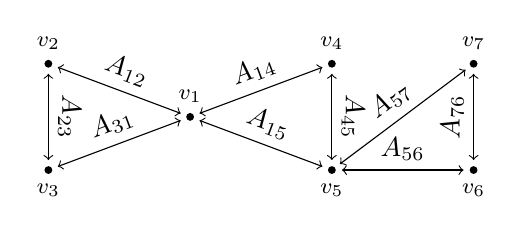
\begin{tikzpicture}[scale=0.9]
		\node [circle,fill=black,inner sep=1pt,label=above:{\footnotesize $v_1$}] (b_i) at (3, 0) {};
		
		\node [circle,fill=black,inner sep=1pt,label=above:{\footnotesize $v_2$}] (b_j) at (1, 0.75) {};
		

		\node [circle,fill=black,inner sep=1pt,label=below:{\footnotesize $v_3$}] (b_l) at (1, -0.75) {};
        \node [circle,fill=black,inner sep=1pt,label=above:{\footnotesize $v_4$}] (b_g) at (5, 0.75) {};
        \node [circle,fill=black,inner sep=1pt,label=below:{\footnotesize $v_5$}] (b_q) at (5, -0.75) {};
	    
        \node [circle,fill=black,inner sep=1pt,label=below:{\footnotesize $v_6$}] (b_y) at (7, -0.75) {};
        \node [circle,fill=black,inner sep=1pt,label=above:{\footnotesize $v_7$}] (b_u) at (7, 0.75) {};

   \path[draw,every node/.style={sloped,anchor=south,auto=false},shorten >=2pt,shorten <=2pt]
		(b_i) edge[<->] node {$A_{12}$}  (b_j)

        (b_j) edge[ <->] node {$A_{23}$} (b_l)
        (b_l) edge[<->] node {$A_{31}$} (b_i)	

        (b_i) edge[<->] node {$A_{14}$} (b_g)
        (b_g) edge[<->] node {$A_{45}$} (b_q)
        (b_i) edge[<->] node {$A_{15}$} (b_q)

        (b_y) edge[<->] node {$A_{56}$} (b_q)
        (b_y) edge[<->] node {$A_{76}$}(b_u)
        (b_u) edge[<->] node {$A_{57}$} (b_q)

		 ;
\end{tikzpicture}
\caption{The graph $\vec{G}$ } 
\label{fig:butterfly_graph}
\end{figure}


% \ebnote{do not give holonomy first}

% Recenltly, notion of holonomy is used to discuss gossip process

% it generated the followiing conditon in the these two given work for tivial and non trivial


% \ebedit{recall holonomy for definition and results}


% these work provide condition but in this work, we proposes an algorithm to contruct 






% \begin{thm}\label{thm:consensus}
% Let $G=(V,E)$ be a simple, connected, bridgeless graph on $n$ nodes with matrix-valued edge weights $A_e$, $e \in E$.  Let  $w^\top \in \operatorname{int}\Delta^{nm-1}$ be such that the set of local stochastic matrices $\{A_{e}\in \mathbb{R}^{nm\times nm}, e \in E\}$ is $w$-holonomic for $G$. Then, for any infinite exhaustive closed walk $\gamma$ in $D_G(w)$, we have that:
% \begin{enumerate}
% \item\label{itm:limit_set} The limit set of ${P}_{\psi(\gamma)}$ is a finite set $\mathcal{L}$. 
% \item\label{itm:block} There exists a relabeling of the nodes such that each element of $\mathcal{L}$ can be expressed as   
% \begin{equation}\label{eqn:limit_set}
% %     P_{\psi(\gamma)} =  \left[  \begin{smallmatrix}
% %         \tilde{P}_{\psi(\gamma)} & 0 \\
% % 0 & M_{\psi(\gamma)} 
% %     \end{smallmatrix} \right]
%     P_{\psi(\gamma)} = \left[\begin{array}{cc}
% \tilde{P}_{\psi(\gamma)} & 0 \\
% 0 & M_{\psi(\gamma)} 
% \end{array}\right] 
% \end{equation}
% where $\tilde{P}_{\psi(\gamma)} $ is a permutation matrix with rows columns indexed by the set $\cap_{C \in \vec{\mathcal{C}}}\pi_{P_C}$ 
% and $M_{\psi(\gamma)}$ is a block diagonal matrix.   
% \item\label{itm:rank_one} The blocks $M_{\psi(\gamma)}^{ii}$ of $M_{\psi(\gamma)}$ are rank-one matrices. 
% \end{enumerate}
% \end{thm}





% In this context, holonomy

% refers to the structure imposed by a set of stochastic matrices on a given weight vector $w$. In particular, when these matrices exhibit finite orbit sets, meaning that iterating the update process results in a cyclic progression through a finite set of weight vectors, this provides a powerful algebraic tool for analyzing the long-term behavior of the system. 


\textbf{Holonomy in the Network.} We employ the concept of holonomy—a powerful algebraic tool that captures the cyclic behavior of weight vector evolution in gossip processes~\citep{chen2022gossip}. 
% In differential geometry, holonomy deals with the variation of some quantity (e.g. a vector) along the loops in a given space~\cite{chen2022gossip}. In our convention, the quantity is a left weight vector, the process evolving the quantity is the gossip process, and the space is the graph $\vec G$. 
For a given cycle $C$ and a weight vector $w$, the process which evolves around the cycle $C$ is said to be $w$-holonomic for $C$ if the weight vector $w$ does not change after completing the cycle (i.e. multiplying by $P_C$) or it does {\em change after completing the cycle} once but comes back to the initial value after completing the cycle finite $k$-times. To be more precise:
% , we have the following definition:

% the weight vector $w$ does not change after completing the cycle (i.e. multiplying by $P_C$) in the graph, the process around the cycle is holonomic on the given weight vector $w$. In addition to that, if there exists a finite $k>1$ such that the weight vector $w$ does {\em change after completing the cycle in the graph} once but comes back to the initial value after completing the cycle $k$-times, the process which evolves the said quantity is called {\em finitely non-holonomic} on the given weight vector $w$. If the process around a cycle $C$ is either holonomic or finitely non-holonomic on the weight vector $w$, it is said to be $w$-holonomic for $C$.

% To be precise, we have the following definition:

%  In differential geometry, holonomy deals with the variation of some quantity (e.g. a vector) along the loops in a given space~\cite{chen2022gossip}. In our convention, the quantity is a left weight vector, the process evolving the quantity is the gossip process, and the space is the graph $\vec G$. 
 
 
%  If there is no variation in this quantity after completing a loop, the process is defined as {\em holonomic}. Otherwise, it is said to be {\em non-holonomic}. 
 
%  In our convention, if there exists a finite $k>1$ such that the quantity does change after completing the loop once but comes back to the initial value after completing the loop $k$-times, the process which evolves the said quantity is called {\em finitely non-holonomic}.
 
 
 % For our purpose, the quantity is a left weight vector, the process evolving the quantity is the gossip process, and the space is the graph $\vec G$. 



% Recent works such as \citep{chen2022gossip} and \citep{bayram2023vector} borrow the notion of holonomy from geometric control. The notion of holonomy in~\cite{bayram2023vector} refers to the structure imposed by a set of stochastic matrices on a given weight vector. In particular, when these matrices exhibit finite orbit sets, meaning that iterating the update process results in a cyclic progression through a finite set of weight vectors, this provides a powerful algebraic tool for analyzing the long-term behavior of the system. Both~\citep{chen2022gossip} and \citep{bayram2023vector} established sufficient conditions, $w$-holonomy, for the convergence of gossip processes to a finite limit set.


\begin{defn}\citep[Holonomic Stochastic Matrices]{bayram2023vector}\label{def:non-trivial} Let $C$ be a cycle in $\vec{G}$ of length greater than $2$ and $w^\top \in \operatorname{int}\Delta^{nm-1}$ be a weight vector. The {\em $w$-order} of $C$ is defined as 
$$
\operatorname{ord}_wC := \min \{k\geq 1: {w}={w}( P_C)^k\},
$$
and $\operatorname{ord}_w C=0$ if the set is empty. The local stochastic matrices $A_{e}$,  $e \in C$,  are said to be \textbf{$w$-holonomic for $C$} if there exists a weight vector $w$ such that $\operatorname{ord}_wC$ is finite and non-zero.
\end{defn}
The local stochastic matrices $A_{e}$ are {\em $w$-holonomic for $G$} if there exists a {\em common} weight vector $w$ so that the $A_e$'s are $w$-holonomic for all $C \in \vec{\mathcal{C}}$ of length greater than $2$. 
% \ebnote{now might need to be updated}.

% When the vector states can be divided into fixed partitions such that each subvector within a partition reaches consensus, the process is characterized as multiple consensus (also known as class-ergodicity). The elements of this partition are referred to as a {\em consensus clusters} ~\cite{bolouki2015consensus,bolouki2013ergodicity,touri2012approximations}.
For a given graph $G = (V, E)$ (satisfying two additional topological conditions: $2$-edge connected and simple), Theorem 1 in \citep{bayram2023vector} shows that if the set of local stochastic matrices $\{A_e , e \in E\}$ is $w$-holonomic for $G$, the infinite product of stochastic matrices associated with the edges in $E$ converges to a limit set with finite cardinality, which depends on the weight vector $w$, provided that an allowable sequence of updates is followed. Note that this result is strong, as it establishes the existence of infinitely many allowable sequences, each of which can be followed in a decentralized manner.
% (see~\cite[Theorem 1]{bayram2023vector} for details).

% Note that this result is a strong notion, as the existence of infinitely many allowable sequences and each allowable sequences can be followed in a decentralized manner, is proven (see~\cite{bayram2023vector} for the details).

% the existence of an allowable sequence that can be followed in a decentralized manner is guaranteed, and the existence of infinitely many allowable sequences is also proven

% In class-ergodic consensus, there exists a partition of the index set. At the limit, the averaging process ensures that the element of each subset reaches a common consensus value independent from other subsets in the partition. 

Let $w=[\alpha^1_1,\alpha^1_2,\cdots,\alpha^1_m,\alpha^2_1,\cdots,\alpha^n_{m-1},\alpha^n_{m}]^\top \in \operatorname{int}\Delta^{nm-1}$ be the given weight vector (by the user) for averaging, where $\alpha^i_k$ denotes the weight assigned to the $k$th entry of agent $i$ at consensus. Let $\{1,\ldots, nm\}$ be a set of indices that label the entries of the weight vector $w$. We say that index $k$ in the index set belongs to an agent, namely agent $i$, if 
$$ (i-1)m +1 \leq k \leq  im.
$$
In this work, we consider that a set $\pi$ is given by the user, $\pi \subset 2^{\{1,\ldots,nm\}}$ is a partition of $\{1,\ldots,nm\}$. We denote by $\pi_a, a=0,\ldots, \ell$, the elements of $\pi$ where $\ell+1$ is the cardinality of $\pi$, also denoted by $|\pi|$. We define the subvector of $w$ induced by the element $\pi_a$ of partition $\pi$ as the vector of dimension $|\pi_a|$, consisting of the entries from $w$ indexed by $\pi_a$, ordered in ascending order. Each subvector is normalized by dividing its entries by their sum, ensuring it is a probability vector in $\operatorname{int}\Delta^{|\pi_a|-1}$. Each element $\pi_a$ of the partition corresponds to a consensus cluster, and the consensus value at the limit is the weighted average of the initial state vector, with weights provided by the subvector of $w$ induced by $\pi_a$.

% Each element of partition $\pi_a$ correspond to cluster consensus and the consus value is the weighte (with rectped t by the subvector of $w$  induced by the element $\pi_a$= the  averaged of states at the limit

% averaging process ensures that the elements of each subset reach weighted average , independent of other subsets in the partition. 


% This normalization guarantees that the weighted average for the consensus clusters is preserved at the limit. When referring to a subvector of $w$ induced by an element $\pi_a$, we assume it is normalized.



% We define the subvector of $w$ induced by the element $\pi_a$ of partition $\pi$ as the vector of dimension $|\pi_a|$, consisting of the entries from $w$ indexed by $\pi_a$, ordered according to the indices in $\pi_a$ in ascending order. Normalization of each subvector of $w$ induced by all elements of partition $\pi$, divided by the sum of all entries, will result in a weighted average for the consensus clusters at the limit. 
% % This normalization ensures that the subvector is also a probability vector in $\Delta^{|\pi_a|-1}$.
% When we refer to a subvector of $w$ induced by an element $\pi_a$ of partition of the index set, we assume it is normalized.



% $\tilde{\pi} = \{\pi_a\}_{a=0}^\ell$ for some $\ell\geq1$.

% In class-ergodic consensus, there exists a partition of the index set such that, at the limit, the averaging process ensures that the elements of each subset reach a common consensus value independent of other subsets in the partition.


% There 

% $\pi$ is given by the user, $\pi \subset 2^{\{1,\ldots,nm\}}$ is a partition of $\{1,\ldots,nm}$. We denote by $\pi_i, i=1,\ldots, \ell$, the elements of $\pi$ where $\ell$ is the cardinality of $\pi$, also denoted by $\|\pi|$.


% Then, in this work, we provide an algorithm to construct a realization of a set of stochastic matrices $\{ A_e \mid e \in E \}$ that is $w$-holonomic for $G$ and leads to consensus clusters for a given partition of the index set ${\pi}$ and a weight vector $w$.

% For example, the graph $G$ in Figure~\ref{fig:butterfly_graph} satisfies the topological conditions. The question, then, is how to construct or find a realization of the stochastic matrices $A_{12}, A_{23}, \dots, A_{75}$ in Figure~\ref{fig:butterfly_graph} for a given $w$ and a partition $\pi = \{1,2,\dots,14\}$ (where $m=2$) such that the infinite product of these matrices converges to a finite limit set, where the consensus clusters correspond to the given partition of indices.

\section{Main Results}

% In this work, we present an algorithm to construct a realization of a set of stochastic matrices $\{ A_e \mid e \in E \}$, for a given partition $\pi$ of the index set and a weight vector $w$, that is $w$-holonomic for $G$ and ensures consensus clusters.





% To address this, we define admissible partitions. 
% To address this,
\textbf{Admissible Partition of Index Set on $G$} We need to test whether a given partition $\pi$ of an index set ensures that the proposed consensus clusters can be realized and that the specified indices can contribute to their respective clusters. Therefore, we introduce the concept of a derived graph to formalize how indices within the same partition remain connected. We then define admissible partition of the index set based on this concept.
% \ebnote{give $\tilde{\pi} = \{\pi_a\}_{a=0}^\ell$ , functional }
% We need the notion of derived graph to define constructible partitions. 
\begin{defn}[Derived Graph $\mathcal{D}^G(\cdot)$ Function]\label{def:derived_graph_w}
Let $G = (V, E)$ be a {matrix-weighted} graph on $n$ nodes. Let $\pi=\{\pi_a\}_{a=0}^\ell$ be a partition of index set. For a given element $\pi_a$ of the partition of the index set $\pi$, the \textit{derived graph of $G$ on the element $\pi_a$ of the partition}, denoted by $\mathcal{D}^G(\pi_a) = (N_{\pi_a}, {E}_{\pi_a})$, is an undirected graph, possibly with multi-edges, where $N_{\pi_a} = \pi_a$. There is an edge $e_{kl} \in {E}_{\pi_a}$ between nodes $k$ and $l$ if one of the following holds:  
\begin{enumerate}
    \item Indices $k$ and $l$ belong to the same agent. 
    \item  There exist $(v_i,v_j) \in E$ where $i$ and $j$ are the agents to which the indices $k$ and $j$ belong, respectively.
        % The agents to which $i$ and $j$ belong are gossiping pairs.
\end{enumerate}
\end{defn}
% Let ${\pi_A}$ be the largest index set among the sets indexing permutation submatrices in $A$; we refer to it as the {\em maximal permutation index of $A$}. 

% Let $\tilde{\pi} = \{\pi_a\}_{a=0}^\ell$ be a partition of the index set $\pi$.

If the derived graph of $G$ on all elements $\pi_a$ of the partition $\pi$, denoted by $\mathcal{D}^G(\pi_a)$, is strongly connected for all $a \in \{0, 1, \dots, \ell\}$, then we call the partition ${\pi}$ an {\em admissible partition on $G$}.

% An admissible partition $\pi$ of an index set ensures that the states whose indices are given by the user contribute to the corresponding consensus cluster.
By using the derived graph, we can verify that there exists a path in $G$ connecting two agents such that every agent on the path has at least two entries whose indices belong to the same proposed consensus cluster. The existence of such a path ensures that information can propagate within the cluster. This approach eliminates the need for direct gossiping between every pair of agents within the cluster. Then, we provide the following example:
% to derive $D^G(\cdot)$ for a given partition of the index set.


% By using the derived graph, we can verify that there exists a path connecting the agents corresponding to each partitioned cluster, allowing the information to propagate within the cluster. This approach eliminates the need for all agent pairs to engage in direct gossiping, instead, it suffices that there exists a path connecting the agents to which the indices belong for a given element of the partition.

% In other words, this definition is particularly useful for determining whether it is possible to propagate information across the graph, rather than requiring all state pairs to engage in direct gossiping. Instead, 
% By introducing the concept of a derived graph, we formalize how indices within the same partitioned cluster remain connected, either through shared agents or through indirect paths via the underlying communication graph.

% The requirement that each derived graph is strongly connected ensures that the partition structure is well-posed for information propagation, making it a valid and meaningful partition of the index set.

% $$
%     \tilde{\pi}
% $$
% \ebnote{partition of ..,}
% $\pi$ is given by the user, $\pi \subset 2^{\{1,\ldots,nm\}}$ is a partition of $\{1,\ldots,nm}$. We denote by $\pi_i, i=1,\ldots, \ell$, the elements of $\pi$ where $\ell$ is the cardinality of $\pi$, also denoted by $\|\pi|$.
 
%  $\pi = \{\pi_a\}_{a=0}^\ell$
%  $\pi_a \subset \{1\,\ldots, nm\}$$
% where $\pi = \cup \pi_a $ $a =0 , n$ 
% } 
% \ebnote{I might draw example derived graph from Fig 1}


\begin{exmp}\label{exmp:derived}  Assume that $n=4$ and $m=2$. Let $G=(V,E)$ be the graph such that $V=\{v_1,v_2,v_3,v_4\}$ and $E=\{(v_1,v_2),(v_2,v_3),(v_3,v_4),(v_4,,v_1)\}$. In words, $G$ is a cyclic graph on $4$ nodes. Consider the partition $\pi = \{{\pi_0} = {\{1,3\}} , {\pi_1} = {\{2,4,5,7\}},{\pi_2}={\{6,8\}}  \}$ is given.  
% $\pi = \{\underbrace{\{1,3\}}_{\pi_0} , \underbrace{\{2,4,5,7\}}_{\pi_1},\underbrace{\{6,8\}}_{\pi_1} \}$ is given. 
% Now, we first check if the partition is admissible. 
% An we have the partition $\pi = \{\underbrace{\{1,3\}}_{\pi_0} , \underbrace{\{2,4,5,7\}}_{\pi_1},\underbrace{\{6,8\}}_{\pi_1} \}$. 
Consider the derived graph $\mathcal{D}^G(\pi_1)$. It consists of four nodes corresponding to indices $\{2,4,5,7\}$. Index $2$ belongs to agent $1$, index $4$ belongs to agent $2$, index $5$ belongs to agent $3$, and index $7$ belongs to agent $4$. Since the graph $G$ contains edges connecting these agents, such as $(v_1,v_2)$ leading to $e_{24} \in E_{\pi_1}$, $(v_2,v_3)$ leading to $e_{45} \in E_{\pi_1}$, $(v_3,v_4)$ leading to $e_{57} \in E_{\pi_1}$, and $(v_4,v_1)$ leading to $e_{27} \in E_{\pi_1}$. It ensures that the derived graph $\mathcal{D}^G(\pi_1)$ is strongly connected (see Figure~\ref{fig:derived_combined}). The derived graph $\mathcal{D}^G(\pi_a)$ is strongly connected for all $a=0,1,2$, which implies that the partition ${\pi}$ is an {\em admissible partition on $G$}

% We repeat the same for the all other elements $\pi_a$ of the partition $\pi$ to see all $\mathcal{D}^G(\pi_a)$ is strongly connected for $a=0,1,2$ (see Figure~\ref{fig:derived_combined})

% Consider the derived graph $D^G(\pi_0)$. It has two nodes corresponding to indices $1$ and $3$. For the element $\pi_0$ of partition $\pi$, index $1$ belongs to agent $1$, and index $3$ belongs to agent $2$. Since there is an edge $v_1v_2 \in E$, an edge exists between nodes $1$ and $3$ in $D^G(\pi_0)$. Thus, the derived graph for $\pi_0$ is strongly connected. 

\begin{figure}
\centering
\begin{tikzpicture}[scale=0.9]
    % Panel 1: D^G(\pi_0)
    \begin{scope}
        \node at (1,1.4) {\footnotesize $\mathcal{D}^G(\pi_0)$};
        
        % Nodes
        \node [circle,fill=black,inner sep=1pt,label=above:{\footnotesize $1$}] (v1) at (1, 0.5) {};
        \node [circle,fill=black,inner sep=1pt,label=below:{\footnotesize $3$}] (v3) at (1, -0.5) {};

        % Edge
        \path[draw,shorten >=2pt,shorten <=2pt]
            (v1) edge[-] node {} (v3);
    \end{scope}

    % Panel 2: D^G(\pi_1)
    \begin{scope}[xshift=3cm]
        \node at (2, 1.4) {\footnotesize $\mathcal{D}^G(\pi_1)$};

        % Nodes
        \node [circle,fill=black,inner sep=1pt,label=above:{\footnotesize $2$}] (v2) at (0, 0) {};
        \node [circle,fill=black,inner sep=1pt,label=above:{\footnotesize $4$}] (v4) at (2, 0.5) {};
        \node [circle,fill=black,inner sep=1pt,label=below:{\footnotesize $5$}] (v5) at (2, -0.5) {};
        \node [circle,fill=black,inner sep=1pt,label=above:{\footnotesize $7$}] (v7) at (4, 0.0) {};

        % Edges
        \path[draw,shorten >=2pt,shorten <=2pt]
            (v2) edge[-] node {} (v4)
            (v4) edge[-] node {} (v5)
            (v5) edge[-] node {} (v7)
            (v2) edge[-] node {} (v7);
    \end{scope}

    % Panel 3: D^G(\pi_2)
    \begin{scope}[xshift=8cm]
        \node at (1, 1.4) {\footnotesize $\mathcal{D}^G(\pi_2)$};

        % Nodes
        \node [circle,fill=black,inner sep=1pt,label=above:{\footnotesize $6$}] (v6) at (1, 0.5) {};
        \node [circle,fill=black,inner sep=1pt,label=below:{\footnotesize $8$}] (v8) at (1, -0.5) {};

        % Edge
        \path[draw,shorten >=2pt,shorten <=2pt]
            (v6) edge[-] node {} (v8);
    \end{scope}
\end{tikzpicture}
\caption{Derived graphs $\mathcal{D}^G(\pi_0)$, $\mathcal{D}^G(\pi_1)$, and $\mathcal{D}^G(\pi_2)$ }
\label{fig:derived_combined}
\end{figure}
%(All Strongly Connected)

\end{exmp}

% Now, we introduce our algorithm to construct set local stochastic matrices $\{A_e, e \in E \}$ such that they are $w$-holonomic for $G$. 

\textbf{Permutation Blocks for $A_e$.} 
From Definition~\ref{def:non-trivial}, we know that some cycles can have $w$-order greater than $1$. In this section, we present a lemma to show that it is sufficient to put a permutation matrix into the state transition matrix of a given cycle $C$ to have the $w$-order of the cycle $C$ is greater than $1$. Note that having $w$-order of a cycle $C$ greater than $1$ is not a necessary condition for having $w$-holonomy for $G$. Therefore, in this section, we provide a design choice for the user by using permutation matrices. 

A stochastic matrix $A$ has {\em a permutation block for an index set $\pi_a$} if the principal block submatrix of $A$ with rows/columns indexed by $\pi_a$ is a permutation matrix with dimension ${|\pi_a|}$. Note that we allow local stochastic matrices to have entries as $\{0,1\}$. This might lead to have permutation blocks in local stochastic matrices and lead permutation blocks at limit for certain indices (see~\cite[Theorem 1]{bayram2023vector}) and the state vector entries labeled by these indices do not contribute to weighted average at the limit. 

Given this, we ask the user to fill $\pi_0$ with the indices of the entries of the state vector that are desired to be in the permutation block at the limit (this set can be empty, as will be discussed later). For a non-empty $\pi_0$, we denote by $w_0$ the subvector of a given weight vector $w$ induced by $\pi_0$ and by $\tilde{w}$ the remaining subvector of $w$ (i.e. induced by $\cup_{a=1}^\ell \pi_a$). For a given cycle $C$, we denote by $P$ and $M$ the principal block submatrices of $P_C$ whose entries are indexed by $\pi_0$ and $\cup_{a=1}^\ell \pi_a$, respectively. Then, we have the following lemma:
\begin{lem}\label{lem:P_c_block}
% For a given $C$ in $\vec{\mathcal{C}}$ and ${\pi}$. 
If $P$ is a permutation matrix with order ${|\pi_0|}$ such that $w_0 P \neq w_0 $ and $M$ is a stochastic matrix such that $\tilde w M=\tilde w$, that is, it holds that (up to labelling): 
\begin{equation}\label{eqn:factorization_Pc}
P_C = \begin{blockarray}{ccc}
\pi_0 & \cup_{a=1}^\ell \pi_a \\
\begin{block}{[cc]c}
P & \mathbf{0} & \pi_0 \\
\mathbf{0} & M & \cup_{a=1}^\ell \pi_a \\
\end{block}
\end{blockarray},
\end{equation}
then the $w$-order of the cycle $C$ is strictly greater than $1$. 
% where $P$ is a permutation matrix with order ${|\pi_0|}$ such that $w_0 P_C \neq w_0 $ and it holds that $\tilde w M=\tilde w$, then the $w$-order of the cycle $C$ is strictly greater than $1$.
\end{lem}

% We need another lemma before discussing their implication.
% \begin{prop}\label{prop:A_e_perm}
% For a given walk $\gamma$ in $G$, if a state transition matrix $P_\gamma$ has a permutation block for some index set $\bar{\pi}$, then, the local stochastic matrix $A_e \in \mathbb{R}^{nm \times nm}$  for all $e \in \gamma$ has a permutation block for the same index set $\bar{\pi}$
% % the rows/columns of $A_e$, for all $e \in \gamma$, corresponding to the indices in the element of index set $\bar{\pi}$ form a permutation block matrix.
% \end{prop}


\begin{rem}
The block structure given in the lemma is also a necessary condition for having $\operatorname{ord}_w C>1$, as discussed in~\citep[Lemma 14]{bayram2023vector}. However, here we only need to show that it is sufficient.
\end{rem} 

% In simpler terms,

See the Section~\ref{sec:proof} for the proof of Lemma~\ref{lem:P_c_block}. Paraphrasing the statements says that if the matrix $P_C$ for a given cycle $C$ have a permutation block such that ${w}_0$ is not fixed point of $P_C$ and the remaining principal submatrix has a left eigenvector $\tilde{w}$ corresponding to eigenvalue $1$, then the $w$-order of the cycle $C$ is strictly greater than one. Furthermore, by construction, it holds $\tilde{w}M^k=\tilde{w}$ for any $k \in \mathbb{N}$. Therefore, we call the block $M$ {\em invariant blocks of $P_C$}. 



Note that if the set $\pi_0$ is empty (by user's decision), then by the definition of subvector, we have $\tilde{w} = w$ and $P_C=M$. We consider only the construction of invariant blocks, which leads to $\operatorname{ord}_w C$ is $1$, (i.e. $wP_C=w)$. 


  



% See that if $\pi_0$ is empty (by user decision), then by the definition of subvector, we have $\tilde{w} = w$.

% he order of $w$ is one and we only consier the co
% and such a matrix $S$ is not exist. Then,we can only conser construction of invariant Eigenspace blocks 


% we

% so the order of $w$ is one, from Definition~\ref{def:non-trivial}.


% See that if $\pi_0$ is emptpy ,then by defitnoi of subvecot we have      #\tilde{w}=w, so the $w$ order is one from Defiton~\ref{def:non-trivial}

% We will show in the next section if $\pi_0$ is emptpy, we can only conser (construction of invariant Eigenspace blocks) of the statement ( and it leads 


% % From Definition~\ref{def:non-trivial}, for a given $w$, we know that $w=wP_C^k$ should for some $k$ for all $C \in G$. 

% The first part of this statement (construction of a permutation matrix) is straightforward, while the latter (construction of invariant Eigenspace blocks) requires careful attention to ensure that the $w$-holonomic condition is satisfied for all cycles in $G$ for given weight vector $w$. 




%  The first part of this statement (construction of a permutation matrix) is straightforward, while the latter (construction of invariant Eigenspace blocks) requires an attention to augrarntee $w$-holnomo condiotn is satifies for all cycle in $G$ for the given weight vector $w$. 
% In the next section, we provide the algorithm to construct the set of stochastic matrices $\{A_e, e \in G\}$ that share the subvector of $w$ induced by $\pi \setminus \pi_0$, as the right eigenvector corresponding to the eigenvalue $1$ for every cycle $C$ in the graph $G$. Then, we can obtain set of lcoal stochiasm amtirces that are $w$ honomolci for graph $g$ (see Defintion~\ref{def:non-trivial})




% Then the following lemma shows that, in order to achieve a permutation matrix at the state transition matrix $P_C$ for certain indices, we must have a permutation block for those index sets at $A_e, \forall e \in C$.
%     . From Proposition~\ref{prop:A_e_perm} and Lemma~\ref{lem:P_c_block}, it is sufficient to put a permutai matrix for teh index set $\pi_0$ for each $A_e$, $e\in C$ and having fixed righe eigenvector block matrix such that the subvector of $w$ labelled by $\pi \setminus \pi_0$ is right eigenvector of $M$ corresponding to eigenvalue $1$ for $w$-honomoy condition. 

 
% Ğraphing the statement says 
% that the rows/columns of $A_e$, for all $e \in \gamma$, corresponding to the indices in the element of index set $\bar{\pi}$ form a permutation block matrix.


% Paraphing the statement says that the rows/columns of $A_e$, for all $e \in \gamma$, corresponding to the indices in the element of index set $\bar{\pi}$ form a permutation block matrix.









% Paraphrasing the statement says thatthe rows/columns of $A_{v_iv_j}$ correspond to the indices in the element of the partition $\pi_0$ is permtuaiton block matrix.
% We will provide the proof in later section now. 

% Now, first consiser $\pi_0$ i

% \begin{lem}
%     For a given constructible partition $\tilde{\pi}$ of $\pi$, the local stochastic matrix $A_{v_iv_j}$ for each edge $v_iv_j$ has permutation block structures corresponding to the indices of the agents $i$ and $j$ in the partition $\pi_0$. 
%     \end{lem}



% for a given 

% This result provide a similar notation with~\citep{bolouki2015consensus,touri2010ergodicity} where these 







% Note that the definition of holonomy is independent from the basepoint of $C$ in $\vec{G}$. We observe that if ${w} = {w} ({P}_{C})^k$ holds for some positive integer $k$, then ${w}={w} ({P}_{C})^{nk}$ holds for all $n \in \Nset$, thus making the set of integers $k$ for which ${w} = {w} ({P}_{C})^k$ holds of infinite cardinality.








% \begin{prop}
% For a given weight vector $w$, let $C$ be a cycle with nonzero $w$-order. Then, there exist a partition of index set $\pi^C$ and there exists a permutation matrix $P$ such that it holds
% \begin{equation}\label{eqn:factorization_Pc}
%   P P_C P^{-1} =\!\begin{blockarray}{ccccc}
% \pi^C_0     & \pi^C_1 & \cdots  & \pi^C_m    &  \\
% \begin{block}{[cccc]c}
% B^{00}_C    &          &        & \textbf{0} & \pi^C_0 \\
%             & B^{11}_C &        &            & \pi^C_1 \\
%             &          & \ddots &            & \vdots \\
% \textbf{0}  &          &        & B^{mm}_C   & \pi^C_m  \\
% \end{block}
% \end{blockarray}%
% \end{equation}
% (up to relabelling) where the principal submatrix $B^{00}_C$ is a permutation matrix and the principal submatrix are $B^{jj}_C$ are irreducible matrix for $j\geq1$
% \end{prop}

% \ebnote{give explannation}

% Paraphsing the statement says that  The following result states that the state traidnon matric for the cycle $C$

% In this section, we provide an algorithm to construct the set of stochastic matrices $\{A_e \mid e \in G\}$ such that each local stochastic matrix $A_e$ satisfies the following: the subvector of $w$ induced by $\pi_a$ is a left eigenvector of the submatrix block in each $A_e$, corresponding to the rows/columns indexed by the elements of partition $\pi_a$.


\textbf{Invariant Blocks for $A_e$.} In this section, we provide an algorithm to construct the set of stochastic matrices $\{A_e \mid e \in G\}$ such that each local stochastic matrix $A_e$ ensures that the subvector of $w$ induced by $\pi_a$ is a left eigenvector corresponding to eigenvalue $1$ of the principal block submatrix of each $A_e$ whose entries indexed by the element $\pi_a$ of partition $\pi$ for all $a = 1, \cdots, \ell$. {We define a mapping $$\Psi: (i, k) \mapsto (i-1)m + k$$ that associates the entry $k \in \{1, \dots, m\}$ of the agent $i \in \{1, \dots, n\}$ with the corresponding each index $\ell\in \{1,2,\cdots,nm\}$.} We denote $nm$-by-$nm$ square matrix with $1$ at the $ij$th entry and $0$ elsewhere by $E_{ij}$. We introduce the definition of the rate matrix set:
% in the space of row stochastic matrices. 
\begin{defn}[Rate Matrix Set on $w$]\label{def:rms}
Let  $\mathcal{B}^{ij}_{kl}(w)$ be the set of $nm \times nm$ stochastic matrices for the $k$th entry of the agent $i$ and the $l$th entry of the agent $j$ such that, for all \( B \in \mathcal{B}^{ij}_{kl}(w) \), it satisfies  
\begin{align}\label{eqn:rms}\\[-2em]
     B = &(1-\beta_1) E_{\Psi(i,k),\Psi(i,k)} +  \beta_1 E_{\Psi(i,k),\Psi(j,l)} + \beta_2 E_{\Psi(j,l),\Psi(i,k)} \nonumber \\
        &+ (1 - \beta_2) E_{\Psi(j,l),\Psi(j,l)} + \sum_{g \neq \Psi(i,k),\Psi(j,l)} E_{g,g}\nonumber
\end{align}
where the parameters satisfy  ${\beta_1}/{\beta_2} = {\alpha^j_l}/{\alpha^i_k}$ with $\beta_1, \beta_2 \in (0,1).$
\end{defn}



% In the this section, we provide an algorithm to construct the set of stochastic matrices $\{A_e \mid e \in G\}$ such that each local stochastic matrices $A_e$ 

% the subvector of $w$ induced by $\pi_a$ is a left egeivne vector to the sub amtrix block in in each $A_e$correspond to rows/colus idnexed by an nidecs elemnt of pariotn $\pi_a$ 



%  each block submatrix in each $A_e$correspond to rows/colus idnexed by an nidecs elemnt of pariotn $\pi_a$ has 
 
%  a right evecof vecot rcorrespnd eigenvcalue $1$ 


% the subvector of $w$ induced by $\cup_{a=1}^\ell \pi_a$ 

% that share the subvector of $w$ induced by $\cup_{a=1}^\ell \pi_a$  the right eigenvector corresponding to the eigenvalue $1$ for every cycle $C$ in the graph $G$ 


% while for each block correspond to rows/colus idnexed by an nidecs elemnt of pariotn $\pi_a$


% Then, we obtain a set of local stochastic matrices that are $w$-holonomic for the graph $G$ (see Definition~\ref{def:non-trivial}). 


% In this subsection, we provide a method to explicitly construct the set of local stochastic matrices  $\{ A_e \in \mathbb{R}^{nm\times nm},\forall e \in E\}$ that $w$-order of cycle is $1$. 
% Let $w=[\alpha^1_1,\alpha^1_2,\cdots,\alpha^1_m,\alpha^2_1,\cdots,\alpha^n_{m-1},\alpha^n_{m}]^\top \in \operatorname{int}\Delta^{nm-1}$ be the weight vector $w$ is given for the convergence where $a^i_l$ is the weight of $l$th state of $i$th agent in the network. 



% Let $\pi \subseteq \{1,\ldots, nm\}$ be a set of indices that label the entries of the weight matrix $w$. 



% Then, we provide an algorithm to find a realization of a set local stochastic matrix $\{A_e, e \in G\}$ for a given graph $G$ and  as a function of $w$ and an admissible partition $\pi$ of the index set, ensuring the set is $w$-holonomic $G$

% ensuring that $w = wP_C^k$. Specifically, we present an algorithm to construct a stochastic matrix from a given probability vector for any state dimension $m$.


% Consider that the weight vector $w$ is given for the convergence. 




% To be more precise, \ebedit{we define a mapping $\Psi: (i, k) \to (i-1)m + k$ that associates agent $i \in \{1, \dots, n\}$ and state $k \in \{1, \dots, m\}$ with the corresponding each index $\ell \in \pi$. }


% \begin{defn}[Rate Matrix Set]
% Let $\mathcal{B}(r)$ be the set of $2$-by-$2$ stochastic matrices, defined as follows:
% \begin{align}
%     \mathcal{B}(r) = \{ \begin{bmatrix}
% 1-\beta_1 & \beta_1  \\
% \beta_2 & 1-\beta_2
% \end{bmatrix}  \in \Delta^{2 \times 2}  :   r= \frac{\beta_1}{\beta_2} ; \beta_1,\beta_2 \in (0,1) \}
% \end{align}
% % with $\beta^1$ and $\beta^2$ real numbers in the open interval $(0,1)$.
% % $$
% % B:=\begin{bmatrix}
% % 1-\beta_1 & \beta_1  \\
% % \beta_2 & 1-\beta_2
% % \end{bmatrix}
% % $$
% % with $\beta^1$ and $\beta^2$ real numbers in the open interval $(0,1)$. 
% For a given rate $r \in (0,1)$, the matrix $B$ is said to be {\em rate matrix for rate $r$} if $B \in \mathcal{B}(r)$. 
% % it holds that 
% % $$
% %     \frac{\beta_1}{\beta_2} = r.
% % $$
% \end{defn}



% \begin{defn}[Rate Matrix Set]
% Let $\mathcal{B}(r)$ be the set of $2$-by-$2$ stochastic matrices, defined as follows:
% \begin{align}
%     \mathcal{B}(r) = \{ \begin{bmatrix}
% 1-\beta_1 & \beta_1  \\
% \beta_2 & 1-\beta_2
% \end{bmatrix}  \in \Delta^{2 \times 2}  :   r= \frac{\beta_1}{\beta_2} ; \beta_1,\beta_2 \in (0,1) \}
% \end{align}
% % with $\beta^1$ and $\beta^2$ real numbers in the open interval $(0,1)$.
% % $$
% % B:=\begin{bmatrix}
% % 1-\beta_1 & \beta_1  \\
% % \beta_2 & 1-\beta_2
% % \end{bmatrix}
% % $$
% % with $\beta^1$ and $\beta^2$ real numbers in the open interval $(0,1)$. 
% For a given rate $r \in (0,1)$, the matrix $B$ is said to be {\em rate matrix for rate $r$} if $B \in \mathcal{B}(r)$. 
% % it holds that 
% % $$
% %     \frac{\beta_1}{\beta_2} = r.
% % $$
% \end{defn}



% for any $B \in \mathcal{B}^{ij}_{kl}(w)$, it holds that 
% \begin{align}
%      B= &(1-\beta^1) {E_{\Psi(i,k),\Psi(i,k)}} +  \beta^1 {E_{\Psi(i,k),\Psi(j,l)}} \\
%         &+ \beta^2 {E_{\Psi(j,l),\Psi(i,k)}} + (1 - \beta^2) {E_{\Psi(j,l),\Psi(j,l)}} \\
%         &+ \sum_{g \neq \Psi(i,k),\Psi(j,l)} E_{g,g}
% \end{align}
% where $\beta^2/\beta^1 = \alpha^j_l /\alpha^i_k$ and $\beta^1,\beta^2 \in (0,1)$

% \end{defn}





% \begin{multline}
%         B^{ij}_{kl} = (1-\beta^{ij}_{kl}) {E_{(i-1)m+k,(i-1)m+k}} +  \beta^{ij}_{kl} {E_{(i-1)m+k,(j-1)m+l}} +
%     \beta^{ji}_{kl} {E_{(j-1)m+l,(i-1)m+k}} + \\ 
%     (1 - \beta^{ji}_{kl}) {E_{(j-1)m+l,(j-1)m+l}} + \sum_{g \neq (i-1)m+k,(j-1)m+l} E_{g,g}
% \end{multline}


% For instance, consider Example~\ebnote{refer to image}

Paraphrasing Definition~\ref{def:rms} says that the principal $2$-by-$2$ submatrix ,corresponding to the $k$th entry of the agent $i$ and the $l$th entry of the agent $j$, of a matrix in $\mathcal{B}^{ij}_{kl}(w)$  is given by 
\begin{align*}\\[-2em]
  \begin{bmatrix}
1-\beta_1 & \beta_1  \\
\beta_2 & 1-\beta_2
\end{bmatrix}  \mbox{ such that } \beta_1/\beta_2 = {\alpha^j_l}/{\alpha^i_k} \\[-2em]
\end{align*}
and the complementary principal submatrix of $B$ is the identity matrix $I_{2m-2}$. 

From \cite[Proposition 6]{chen2022gossip}, we know that for any pair of $\alpha^i_k, \alpha^j_l \in (0, 1)$, the set of rate matrices is non-empty, that is, there exists a rate matrix on every $w \in \operatorname{int} \Delta^{nm-1}$. One can easily see that there are infinitely many tuples $(\beta_1, \beta_2)$ satisfying the condition for fixed $(\alpha^j_l,\alpha^i_k)$.
A stochastic matrix $B$ constructed by~\eqref{eqn:rms} has one degree of freedom due to the constraint $\alpha^i_k \beta_1 = \alpha^j_l \beta_2$. Then, the set $\mathcal{B}^{ij}_{kl}(w)$ forms a one-dimensional manifold (which can be interpreted as a curve in the space of stochastic matrices) in the space of $nm \times nm$ matrices (which is an ambient space of $2nm$ dimensions).

% , it forms a one-dimensional manifold—which can be interpreted as a curve in the space of stochastic matrices. 

% that there are infinitely many tuples $(\beta_{1} ,\beta_{2} )$ which satisfies condition for a given fixed $\alpha^3_1/\alpha^1_2$. A general $2 \times 2$ stochastic matrix has two degrees of freedom, since each row sums to $1$, and we are left with two independent parameters: $\beta_1$ and $\beta_2$. However, these parameters are constrained by the equation: $\alpha^i_k \beta_1 = \alpha^j_l \beta_2$. This introduces a one-degree-of-freedom constraint on $(\beta_1, \beta_2)$, reducing the dimensionality of the set. 


% There are infinitely many tuples $(\beta_1, \beta_2)$ satisfying the condition for a fixed $\alpha^3_1/\alpha^1_2$. A $2 \times 2$ stochastic matrix has two degrees of freedom, but the constraint $\alpha^i_k \beta_1 = \alpha^j_l \beta_2$ reduces it to one.

% Since the set $\mathcal{B}^{ij}_{kl}(w)$ is one-dimensional in the space of $2 \times 2$ matrixes (which is a $2nm$-dimensional ambient space),it forms a one-dimensional manifold—which can be interpreted as a curve in the space of stochastic matrices. 

% From \cite[Proposition 6]{chen2022gossip}, we know that for any pair of $\alpha^i_k,\alpha^j_l \in (0,1)$ , the rate matrix set is nonempty, that is, there exist a rate matrix for every $w \in \operatorname{int}\delta^{nm-1}$  

% \ebnote{recall chen paper for surjective}

% Now, we provide the defition of constructor set of local stochastic matrices will be core of our algorithm. 

% \begin{defn}[Constructor Set of Local Stochastic Matrices]  
% Let $ v_i $ and $ v_j $ be a gossiping pair in $ \vec{G} $. For a given weight vector $ w $ and a given patition of index set $\tilde{\pi}={\pi_a}_{a=0}^\ell$, we define the {\em constructor set} of the local stochastic matrix $ A_{v_i v_j} $ for $ w $ denoted by $ \Phi^{ij}(w) $, as a set satisfying:  
% $$
% \Phi^{ij}(w) = \bigcup_{a=1}^{\ell} \{  \mathcal{B}^{ij}_{kl}(w) \mid \Psi((i,k)) \in \pi_a  \land  \Psi((j,l)) \in\pi_a   \}
% $$
% such that for every pair \(\Psi((i,k)), \Psi((j,l)) \) in the same element of partition of index set, there exists at least one matrix \( A \in \Phi^{ij}(w) \) with \( A \in \mathcal{B}^{ij}_{kl}(w) \) if . Furthermore, \(\Phi^{ij}(w)\) does not contain any matrix outside the family \(\mathcal{B}^{ij}_{kl}(w)\), though it may contain multiple elements from the same \(\mathcal{B}^{ij}_{kl}(w)\).  
% \end{defn}

% \begin{rem}
% Note that the constructor set of local stochastic matrices omits the elements of the partition set corresponding to the permutation block $\pi_0$. 
% \end{rem}




% Paraphsing the sttament says that for a gossping pair, $\Phi^{ij}(w)$ we collect 


% \begin{defn}[Constructor Set of Stochastic Matrices]
% Let $v_i$ and $v_j$ be a gossiping pair in $\vec{G}$. For a given weight vector $w$, we define constructor set of local stochastic matrix $A_{v_iv_j}$ for $w$, denoted by $\Phi^{ij}(w)$, as a set that consists of least an element from the set $\mathcal{B}^{ij}_{kl}(w)$ for every pair of $(k,l)$. To be more precies,
% \end{defn}


% \ebnote{change it make it dpeedneing on partition}


% \begin{equation}\label{eqn:factorization_Pc}
% M=\left[\begin{blockarray}{cccc|ccc|cccc}
%  & 1 & & & & & & & \\
%  \begin{block}{[cccccccccc]c}
% & & \ddots  & & & & & & \\
%  &  &  & 1 & & & & & &\\
% \beta &  &  &  & \alpha& & & & &\\
% \hline & & & & & & & & &\\
% & & & & &  \ddots  & & & &\\
% & & & &  & & & \alpha & &\\
% \hline & & & & & & & & 1 & \\
%  & &   & & & & & & & \ddots \\
%  &  &  &  & & & & & & & 1\\
%  \gamma &  &  &  & & & & \beta & &\\
%  \end{block}
% \end{blockarray}\right],
% \end{equation}

%  \begin{equation}\label{eqn:factorization_Pc}
%   B=\begin{blockarray}{cccccc}
% 1     &  \cdots & m  & \cdots  & \pi^C_m    &  \\
% \begin{block}{[ccc|cc]c}
% 1-\beta_1    &    &      &        & \textbf{0} & 1 \\
%           & B^{11}_C &    &    &            & \vdots \\
%             &    &      & \ddots &            & m \\
% \textbf{0}  &    &      &        & B^{mm}_C   & \pi^C_m  \\
% \end{block}
% \end{blockarray}%
% \end{equation}







% Let $C=v_1v_2\cdots v_\ell$ be a cycle in $\vec{G}$. We construct set of local stochastic matrices $\{ A_e \in \mathbb{R}^{nm\times nm},\forall e \in C\}$ such that it holds
% $$
%     w = w P_C
% $$
% where $P_C = A_{v_1v_2}A_{v_2v_3}\cdots A_{v_{\ell-1}v_{\ell}}$.

% A stochastic matrix $ A_{ij} $ is said to be {}

% Let \( A_{ij} \) be a matrix formed by the product of a finite sequence of distinct matrices selected from \( \Phi^{ij}(w) \), i.e.,  \[
% A_{ij} = \phi_1 \phi_2 \dots \phi_r,
% \]
% where \( \phi_1, \phi_2, \dots, \phi_r \) are chosen {\em without replacement} from \( \Phi^{ij}(w) \), meaning that each matrix appears at most once in the product. The order of multiplication is arbitrary but fixed for a given realization.  


% Now, we can present the numerical algorithm to contruct a local stochastic matrix..
% Now, we are in a position to state the algorithm. 
% to find a realization of a set of local stochastic matrices ${A_e, e \in G}$ for a given graph $G$, as a function of $w$ and an admissible partition $\pi$ of the index set, ensuring that the set is $w$-holonomic for $G$.
\textbf{Algorithm.} Now, we can present Algorithm~\ref{alg:state_transition}.
\begin{algorithm}
\caption{Construction of a local stochastic matrix \( A_{ij} \) for a given partition ${\pi}$ and a given weight vector $w$}\label{alg:state_transition}
\begin{algorithmic}
\STATE \textbf{Input:} $ {\pi}=\{ \pi_a \}_{a=0}^\ell, w , \{i,j\} \gets v_iv_j$ % \gets v_iv_j$ %\COMMENT{Weight vector}
% \STATE \textbf{Input 2:} $\tilde{\pi}=\{ \pi_a \}_{a=0}^\ell$ %\COMMENT{Partition of Index Set}
% \STATE \textbf{Input 3:} $e=v_iv_j$
\STATE \textbf{Output:} \( A_{ij} \)
\STATE \textbf{Initialize} \( A_{ij} = I \) %(Identity matrix) 
\STATE $\triangleright  \mbox{Loop for the elements $\pi_a$ of partition }$

\FOR{$a = 1 \text{ to } \ell$}  
    \STATE $\triangleright  \mbox{Loop over the entries of the agent } i$
    \FOR{$k = 1 \text{ to } m$}  
        \STATE $\triangleright  \mbox{Loop over the entries of the agent } j$
        \FOR{$l = 1 \text{ to } m$}
        % \FOR{$l = 1 \text{ to } m$}
                 % \IF{$\Psi((i,k)) \in\pi_a  \land  \Psi((j,l)) \in\pi_a $}
            \IF{$(i-1)m + k  \in\pi_a  \mbox{ and } (j-1)m + l  \in\pi_a $}
                \STATE $ \alpha^j_l \gets w[(j-1)m + l] $ 
                \STATE $ \alpha^i_k \gets w[(i-1)m + k] $ 
    
                % \algorithmiccomment{ Determine the weight parameters \( \alpha^j_l \) and \( \alpha^i_k \) from the weight vector \( w \), where \( \alpha^j_l \) corresponds to state \( l \) in agent \( j \) and \( \alpha^i_k \) corresponds to state \( k \) in agent \( i \).}
                \STATE \( r \gets {\alpha^j_l}/{\alpha^i_k} \)
                % \STATE \textit{Construct} a stochastic matrix matrix \( \mathcal{B}(r) \)
                % \[
                % \mathcal{B}(r) =  \begin{bmatrix} 1 - \beta_1 & \beta_1 \\ \beta_2 & 1 - \beta_2 \end{bmatrix} : r = \frac{\beta_1}{\beta_2}, \, \beta_1, \beta_2 \in (0, 1) \right\}.
                % \]
                \STATE Pick $\beta_1$ and $\beta_2$ 
                 such that $\beta_1 / \beta_2 = r$ with $\beta_1,\beta_2 \in (0,1)$
                \STATE Get a matrix $B^{ij}_{kl} \in \mathcal{B}^{ij}_{kl}(w)$ via equation~\eqref{eqn:rms} 
                % for selected $\beta_1$,$\beta_2$ and given pair $(j,l)$ and $(i,k)$
                % \STATE Construct a rate matrix for agent $i$ state $k$, $\alpha^i_k$, and agent $j$ state $l$, $\alpha^j_l$ (See Definition~\ref{def:rms})
                % \STATE  \hspace{1cm} \( \phi \in  \mathcal{B}^{ij}_{kl}(w) \)
            %             \STATE Construct a stochastic matrix \( \bar{B}^{ij}_{kl} \in  \mathcal{B}(r) \):
            % \[
            %  \bar{B}^{ij}_{kl}  =  \begin{bmatrix} 1 - \beta_1 & \beta_1 \\ \beta_2 & 1 - \beta_2 \end{bmatrix}, \quad r = \frac{\beta_1}{\beta_2}, \quad \beta_1, \beta_2 \in (0, 1).
            % \]
    
            %     % \STATE \textit{Select} one matrix \( \bar{B}^{ij}_{kl} \in \mathcal{B}(r) \) for the current pair \( (k, l) \).
            %     \STATE Construct the matrix \( \phi_{kl} \) by embedding \( \bar{B}^{ij}_{kl} \) as the principal \( 2 \times 2 \) submatrix corresponding to rows/columns $\Psi((j,l))$ and $\Psi((i,k))$ , and set the complementary \( (2m - 2) \times (2m - 2) \) submatrix as the identity matrix \( I_{2m-2} \)
                \STATE Update the stochastic matrix:
                \STATE \hspace{1cm} \( A_{ij} \gets A_{ij} \cdot B^{ij}_{kl} \)
            \ENDIF
        \ENDFOR
    \ENDFOR
\ENDFOR
\RETURN $A_{ij}$
\end{algorithmic}
\end{algorithm}


\begin{rem}\label{rem:perm}
Note that the algorithm starts iterating from the element $\pi_1$ (that is, it ignores the element $\pi_0$ of the partition corresponding to the permutation block). Once the user decides to have permutation block at the limit (i.e. non-empty $\pi_0$), it is sufficient to place a (non-identity)  permutation matrix in the principal block submatrix of $A_{ij}$, whose entries are indexed by all $k$ and $l$ such that $\Psi(i,k) \in \pi_0$ and $\Psi(j,l) \in \pi_0$ such that the subvector of $w$ induced by $\pi_0$ is not a fixed point of this submatrix,(see Lemma~\ref{lem:P_c_block}). 
\end{rem}

\begin{thm}[Correctness of Algorithm~\ref{alg:state_transition}]\label{thm:holonomic}
% Let $C = v_1 v_2 \cdots v_\ell$ be a cycle in $\vec{G}$, and 
Let $G=(V,E)$ be a simple, $2$-edge connected graph on $n$ nodes with matrix-valued edge weights $A_e$, $e \in E$. Let ${\pi}$ be a admissible partition of index set on $G$. Let $\{ A_e \in \mathbb{R}^{nm \times nm} \mid e \in E \}$ be the set of local stochastic matrices constructed using Algorithm~\ref{alg:state_transition}. Then, the set $\{ A_e \in \mathbb{R}^{nm \times nm} \mid e \in E \}$ is $w$-holonomic for $G$. 
% it holds that  
% $$
% w = w P_C,
% $$  
% where $P_C$ is the product of the local stochastic matrices along cycle $C$, that is, $P_C = A_{v_1v_2}A_{v_2v_3}\cdots A_{v_{\ell-1}v_{\ell}}$.  
\end{thm}  
See Section~\ref{sec:proof} for the proof of Theorem~\ref{thm:holonomic}. We now provide an example for the algorithm. 



% \end{exmp}
% Assume that $n=4$ and $m=2$. Let $G=(V,E)$ be the graph such that $V=\{v_1,v_2,v_3,v_4\}$ and $E=\{v_1v_2,v_2v_3,v_3v_4,v_4v_1\}$. In words, $G$ is a cycle graph on $4$ nodes. Consider the partition $\pi = \{\underbrace{\{1,3\}}_{\pi_0} , \underbrace{\{2,4,5,7\}}_{\pi_1},\underbrace{\{6,8\}}_{\pi_1} \}$ is given.

% Now, we first check if the partition is admissible. 


% % An we have the partition $\pi = \{\underbrace{\{1,3\}}_{\pi_0} , \underbrace{\{2,4,5,7\}}_{\pi_1},\underbrace{\{6,8\}}_{\pi_1} \}$. 



% Consider the derived graph $D^G(\pi_0)$. It has two nodes corresponding to indices $1$ and $3$. For the element $\pi_0$ of partition $\pi$, index $1$ belongs to agent $1$, and index $3$ belongs to agent $2$. Since there is an edge $v_1v_2 \in E$, an edge exists between nodes $1$ and $3$ in $D^G(\pi_0)$. Thus, the derived graph for $\pi_0$ is strongly connected. 

% We repeat the same for the all other elment of the partition $\pi$. We get the derived graph as follows: 

% \begin{figure}
% \centering
% \begin{tikzpicture}[scale=0.9]
%     % Panel 1: D^G(\pi_0)
%     \begin{scope}
%         \node at (1,1.5) {\footnotesize $D^G(\pi_0)$};
        
%         % Nodes
%         \node [circle,fill=black,inner sep=1pt,label=above:{\footnotesize $1$}] (v1) at (1, 0.5) {};
%         \node [circle,fill=black,inner sep=1pt,label=below:{\footnotesize $3$}] (v3) at (1, -0.5) {};

%         % Edge
%         \path[draw,shorten >=2pt,shorten <=2pt]
%             (v1) edge[<->] node {} (v3);
%     \end{scope}

%     % Panel 2: D^G(\pi_1)
%     \begin{scope}[xshift=3cm]
%         \node at (2, 1.5) {\footnotesize $D^G(\pi_1)$};

%         % Nodes
%         \node [circle,fill=black,inner sep=1pt,label=above:{\footnotesize $2$}] (v2) at (0, 0) {};
%         \node [circle,fill=black,inner sep=1pt,label=above:{\footnotesize $4$}] (v4) at (2, 0.5) {};
%         \node [circle,fill=black,inner sep=1pt,label=below:{\footnotesize $5$}] (v5) at (2, -0.5) {};
%         \node [circle,fill=black,inner sep=1pt,label=above:{\footnotesize $7$}] (v7) at (4, 0.0) {};

%         % Edges
%         \path[draw,shorten >=2pt,shorten <=2pt]
%             (v2) edge[<->] node {} (v4)
%             (v4) edge[<->] node {} (v5)
%             (v5) edge[<->] node {} (v7)
%             (v2) edge[<->] node {} (v7);
%     \end{scope}

%     % Panel 3: D^G(\pi_2)
%     \begin{scope}[xshift=8cm]
%         \node at (1, 1.5) {\footnotesize $D^G(\pi_2)$};

%         % Nodes
%         \node [circle,fill=black,inner sep=1pt,label=above:{\footnotesize $6$}] (v6) at (1, 0.5) {};
%         \node [circle,fill=black,inner sep=1pt,label=below:{\footnotesize $8$}] (v8) at (1, -0.5) {};

%         % Edge
%         \path[draw,shorten >=2pt,shorten <=2pt]
%             (v6) edge[<->] node {} (v8);
%     \end{scope}
% \end{tikzpicture}
% \caption{Derived graphs $D^G(\pi_0)$, $D^G(\pi_1)$, and $D^G(\pi_2)$ (All Strongly Connected)}
% \label{fig:derived_combined}
% \end{figure}


% \end{exmp}


% \begin{figure}
% \centering
% \begin{tikzpicture}[scale=0.9]
%     % Left graph (D^G(\pi_0) and D^G(\pi_2))
%     \begin{scope}
%         % Nodes for D^G(\pi_0)
%         \node [circle,fill=black,inner sep=1pt,label=above:{\footnotesize $1$}] (v1) at (0, 0.5) {};
%         \node [circle,fill=black,inner sep=1pt,label=above:{\footnotesize $3$}] (v3) at (2, 0.5) {};

%         % Nodes for D^G(\pi_2)
%         \node [circle,fill=black,inner sep=1pt,label=above:{\footnotesize $6$}] (v6) at (0, -0.5) {};
%         \node [circle,fill=black,inner sep=1pt,label=above:{\footnotesize $8$}] (v8) at (2, -0.5) {};

%         % Edges
%         \path[draw,shorten >=2pt,shorten <=2pt]
%             (v1) edge[<->] node {} (v3)
%             (v6) edge[<->] node {} (v8);
%     \end{scope}

%     % Right graph (D^G(\pi_1))
%     \begin{scope}[xshift=5cm]
%         % Nodes
%         \node [circle,fill=black,inner sep=1pt,label=above:{\footnotesize $2$}] (v2) at (0, 0.5) {};
%         \node [circle,fill=black,inner sep=1pt,label=above:{\footnotesize $4$}] (v4) at (2, 0.5) {};
%         \node [circle,fill=black,inner sep=1pt,label=below:{\footnotesize $5$}] (v5) at (2, -0.5) {};
%         \node [circle,fill=black,inner sep=1pt,label=above:{\footnotesize $7$}] (v7) at (4, 0) {};

%         % Edges
%         \path[draw,shorten >=1pt,shorten <=1pt]
%             (v2) edge[<->] node {} (v4)
%             (v4) edge[<->] node {} (v5)
%             (v5) edge[<->] node {} (v7)
%             (v2) edge[<->] node {} (v7);
%     \end{scope}
% \end{tikzpicture}
% \caption{Derived graphs $D^G(\pi_0)$, $D^G(\pi_1)$, and $D^G(\pi_2)$ (All Strongly Connected)}
% \label{fig:derived_combined}
% \end{figure}




% for $\pi_1$ index $2$ belongs to agent $1$, $4$ belong to agent $2$, $5$ belong to agent $3$, $7$ belong to agent $4$

% there is an edge between all like $v_1v_2$ for,  so the derived graph for $\pi_0$ is SCC


% for $\pi_2$ index $6$ belongs to agent $3$, $8$ belong to agent $4$,

% there is an edge between all so $v_1v_2$ so the derived graph for $\pi_0$ is SCC










% Now consider $e=v_1 v_2$, then for $k=1$ is not in $\pi_1$ 

% $k=2$ (correspond to index $2$) and $l=2$ (corerpsonf to $4$) 
% it is 
% we have $\alpha^1_2 = 0.209$ and $\alpha^2_2=0.027$ 
% rate rate is $r=0.129$ then by using it we select $\beta_1= 0.082$ and $\beta_2= 0.630$, isince $ \beta_1/\beta_2=0.129 $
% then, we have $B^{12}_{22}$

\begin{exmp}[Cont.] Recall  the graph $G$ and admissible partition $\pi$ of index set on $G$ in Example~\ref{exmp:derived}. 

Let $w=[0.012, 0.209, 0.062, 0.027 , 0.050,
       0.081, 0.013, 0.544]$ be the weight vector given by the user. Now, consider the edge $e = v_1 v_2$. For $k = 1$, we have the index $1$ (where $\Psi(1,1)=1$), which is not in $\pi_1$. So, the condition in Line $10$ of Algorithm~\ref{alg:state_transition} is not satisfied. We pass to $k = 2$ (where $\Psi(1,2)=2$) and $l = 2$ (where $\Psi(2,2)=4$), we have the following values from the weight vector $w$:
\[
\alpha^1_2 = 0.209, \quad \alpha^2_2 = 0.027.
\]
Then, the rate $r =\alpha^2_2/ \alpha^1_2 = 0.129$. Using this rate, we select $\beta_1 = 0.082$ and $\beta_2 = 0.630$, since $\frac{\beta_1}{\beta_2} = 0.129$. By using equation~\eqref{eqn:rms}, we obtain the matrix $B$ as follows:
% $B_1 \in B^{12}_{22}$. 
\begin{align*}
 \mathcal{B}^{12}_{22}(w) \ni B = 
\left[ \begin{smallmatrix} 
1.000 &   &   &   &   &   &   &   \\ 
  & 0.918 &   & 0.082 &   &   &   &   \\ 
  &   & 1.000 &   &   &   &   &   \\ 
  & 0.630 &   & 0.370 &   &   &   &   \\ 
  &   &   &   & 1.000 &   &   &   \\ 
  &   &   &   &   & 1.000 &   &   \\ 
  &   &   &   &   &   & 1.000 &   \\ 
  &   &   &   &   &   &   & 1.000 \\ 
\end{smallmatrix} \right]
\end{align*}
Note that only the principal $2$-by-$2$ submatrix whose entries are indexed by $\{2,4\}$ is different from the identity matrix. For the edge ${v_1v_2}$, there is no other pair that satisfies the condition in Line $10$. Now, we can then check the permutation block. Since the indices corresponding to the permutation block $\pi_0=\{1,3\}$ belong to agent $1$ and agent $2$ (i.e. $\Psi(1,1) = 1 \in \pi_0$ and $\Psi(2,1) = 3 \in \pi_0$), we can place a non-identity permutation matrix in the principal block submatrix of $B$ whose entries are indexed by $\{1,3\}$ (see Remark~\ref{rem:perm}). Then, we have the following final form of the local stochastic matrix: 


% for the given edge $A_{v_1v_2}$ , there is no pair thaat satisfies the condiotn in Line $10$. then we can check teh permtaiot block 


%  now since the indexe correpsond  permtuaiot block $\pi_0$ is belong to agent $1$ and $2$ so, 
%  so we can put an non inde ablock correpsond (see Remark~\ref{rem:perm} to  index $1$ and $3$ since ($\Psi(1,1)=1$ and $\Psi(2,1)=3$ )

\begin{align*}
 A_{12} = 
\left[ \begin{smallmatrix} 
 &   & 1.000  &   &   &   &   &   \\ 
  & 0.918 &   & 0.082 &   &   &   &   \\ 
 1.000 &   &  &   &   &   &   &   \\ 
  & 0.630 &   & 0.370 &   &   &   &   \\ 
  &   &   &   & 1.000 &   &   &   \\ 
  &   &   &   &   & 1.000 &   &   \\ 
  &   &   &   &   &   & 1.000 &   \\ 
  &   &   &   &   &   &   & 1.000 \\ 
\end{smallmatrix} \right]
\end{align*}
\end{exmp}
% In the Example, one can easily verify that we have $w(A_{12})^2=w$ where $wA_{12}=w$

% \ebnote{I might add one more but no necesarry}
% Now consider the edge $e=v_2v_3$. For $k = 2$ (where $\Psi(2,2)=4$) and $l = 1$ (where $\Psi(3,1)=5$), we have:
% \[
% \alpha^2_2 = 0.027 \quad \text{and} \quad \alpha^3_1 = 0.050.
% \]
% The rate is $r = \alpha^3_1 / \alpha^2_2 = 1.840$. Using this, we select $\beta_1 = 0.889$ and $\beta_2 = 0.483$, since $\beta_1 / \beta_2 = 0.129$. By using equation~\eqref{eqn:rms}, we obtain the following matrix $B_1 \in B^{23}_{21}$.

% \begin{align*}
% \mathcal{B}^{23}_{21} \ni B_1 \small
% \left[ \begin{smallmatrix} 
% 1.000 &   &   &   &   &   &   &   \\ 
%   & 1.000 &   &   &   &   &   &   \\ 
%   &   & 1.000 &   &   &   &   &   \\ 
%   &   &   & 0.111 & 0.889 &   &   &   \\ 
%   &   &   & 0.483 & 0.517 &   &   &   \\ 
%   &   &   &   &   & 1.000 &   &   \\ 
%   &   &   &   &   &   & 1.000 &   \\ 
%   &   &   &   &   &   &   & 1.000 \\ 
% \end{smallmatrix} \right]
% \end{align*}


% Note that only the principal $2$-by-$2$
% submatrix corresponding to index $2$ and $4$ is different from a identity matrix.

% Thus, we obtain $B^{23}_{21}$.



% similart we have 




% Now consider $e=v_2 v_3$

% $k=2$ (correspond to index $4$) and $l=1$ (corerpsonf to $5$)
% it is 
% we have $\alpha^2_2 = 0.0271704$ and $\alpha^3_1=0.05000697 $ 
% rate rate is $r=1.8404942003289695$ then by using it we select $\beta_1= 0.889345941502395$ and $\beta_2= 0.48321040150163663$, isince $ \beta_1/\beta_2=0.129 $
% then, we have $B^{23}_{21}$




% \ebnote{change}
% Now consider $e=v_3 v_4$

% $k=1$ (correspond to index $4$) and $l=1$ (corerpsonf to $5$)
% it is 
% we have $\alpha^2_2 = 0.0271704$ and $\alpha^3_1=0.05000697 $ 
% rate rate is $r=1.8404942003289695$ then by using it we select $\beta_1= 0.889345941502395$ and $\beta_2= 0.48321040150163663$, isince $ \beta_1/\beta_2=0.129 $
% then, we have $B^{23}_{21}$

% \begin{align*}
% \mathcal{B}^{23}_{21} \ni B_1 \small
% \begin{pmatrix}
% 1.000 &   &   &   &   &   &   &   \\ 
%   & 1.000 &   &   &   &   &   &   \\ 
%   &   & 1.000 &   &   &   &   &   \\ 
%   &   &   & 0.111 & 0.889 &   &   &   \\ 
%   &   &   & 0.483 & 0.517 &   &   &   \\ 
%   &   &   &   &   & 1.000 &   &   \\ 
%   &   &   &   &   &   & 1.000 &   \\ 
%   &   &   &   &   &   &   & 1.000 \\ 
% \end{pmatrix}
% \end{align*}


% we

% Paraphrasing the Definition~\ref{def:rms} says that the principal $2$-by-$2$ submatrix corresponding to state $l$ in the agent $j$ and the state $k$ in the agent $i$ of a matrix in $\mathcal{B}^{ij}_{kl}(w)$  is given by 
% \begin{equation}
%   \begin{bmatrix}
% 1-\beta_1 & \beta_1  \\
% \beta_2 & 1-\beta_2
% \end{bmatrix}  
% \end{equation}
% where $\beta_1/\beta_2 = \frac{\alpha^j_l}{\alpha^i_k}$ and the complementary principal submatrix of $B$ is the identity matrix $I_{2m-2}$. 

% \ebnote{make it example}
% For example, assume that $n=3$ and $m=2$, then, we have a matrix $B \in \mathcal{B}^{13}_{21}$ for state $2$ in the agent $1$ (cor. to index $2$) and state $1$ in the agent $3$ (corrs. to index $5$) 
% % \ebnote{weird}
% \begin{equation}\label{eqn:factorization_Pc}
%   B =\!\begin{blockarray}{ccccccc}
% 1     & 2 &   3 & 4&  5    & 6 \\
% \begin{block}{[cccccc]c}
%  1 & 0  & 0  & 0 & 0 & 0 &  1  \\ 
%  0 &   1-\beta_1   &  0  & 0 &  \beta_1  & 0 &2 \\
%  0     &  0    & 1  &0  &   0      & 0  & 3 \\
% 0    &   0    &  0& 1 &  0 & 0 & 4 \\
% 0 & \beta_2     &0 &0 &  1-\beta_2 & 0 &  5 \\
% 0 &  0 & 0 & 0 &0   & 1 & 6 \\
% \end{block}
% \end{blockarray}%
% \end{equation} 
% where it holds  that $\beta_1/\beta_2=\alpha^3_1/\alpha^1_2$.

% \begin{align*}
% \small
% \begin{bmatrix}
% 0.76 &   &   &   & 0.24 &   \\ 
%   & 1.00 &   &   &   &   \\ 
%   &   & 1.00 &   &   &   \\ 
%   &   &   & 1.00 &   &   \\ 
% 0.26 &   &   &   & 0.74 &   \\ 
%   &   &   &   &   & 1.00 \\ 
% \end{bmatrix}
% \end{align*}

% \begin{align*}
% \small
% \begin{pmatrix}
% 0.952 & 0.025 &   &   & 0.022 &   \\ 
%   & 0.628 &   &   & 0.372 &   \\ 
%   &   & 1.000 &   &   &   \\ 
%   &   &   & 1.000 &   &   \\ 
% 0.682 & 0.170 &   &   & 0.148 &   \\ 
%   &   &   &   &   & 1.000 \\ 
% \end{pmatrix}
% \end{align*}

% \ebnote{ddelte here and have an example after }
% For example, the graph $G$ in Figure~\ref{fig:butterfly_graph} satisfies the required topological conditions. The key question is how to construct a realization of the stochastic matrices $A_{12}, A_{23}, \dots, A_{75}$ in Figure~\ref{fig:butterfly_graph} for a given $w$ and partition $\pi = {1,2,\dots,14}$ (where $m=2$) such that their infinite product converges to a finite limit set, with consensus clusters aligning with the given partition.


% \begin{algorithm}[htp]
% \caption{ A }\label{alg:state_transition}
% \begin{algorithmic}[1]
% \STATE \textbf{Input:} Constructor set $\Phi^{ij}(w)$  
% \STATE \textbf{Output:} Constructed stochastic matrix $A_{ij}$  
% \STATE Initialize $A_{ij} = I$ (Identity matrix)
% \FOR{$k = 1 \text{ to } r$}
%     \STATE Pick a matrix $\phi_k$ from $\Phi^{ij}(w)$ 
%     \STATE Remove it from the set \textit{without replacement}
%     \STATE Multiply the selected matrix:  
%     \STATE \hspace{1cm} $A_{ij} = A_{ij} \cdot \phi_k$
% \ENDFOR
% \RETURN $A_{ij}$  
% \end{algorithmic}  
% \end{algorithm}




% \ebnote{Here I need explaniton of Theorem and its implications}
\section{Proof of Main Results}\label{sec:proof}
% Let $w_0$ be the subvector of $w$ labelled by $\pi_0$ and  $\tilde{w}$ be the subvector of $w$ labelled by $\pi \setminus \pi_0$. 


% First, we prove the auxiliary resultswe prove the main theorem.

% If $S$ is different from the identity block, then we can relabel the index set such that $S$ becomes the identity. For the given definition of conjugacy, the matrix $S$ implies a conjugate relation between $P_C$ and the block matrix composed of $P$ and $M$, which implies equivalence up to relabeling. Therefore, without loss of generality, if a matrix $S$ exist, then we can assume that $S$ is the identity. 

% Without loss of generality, we can assume $\pi_0$ is the first indeixn in the index set. Then, we have write 
\begin{proof}[Proof of Lemma~\ref{lem:P_c_block}].
We assume that $P$ is a permutation matrix and that $w_0 P \neq w_0$. Then, there exists a finite $k > 1$ such that $P^k = I$, which implies that $w_0 P^k = w_0$. Now, we take the $k$-th power of~\eqref{eqn:factorization_Pc} and multiply both sides by the weight vector $w = [ w_0 , \tilde{w} ]$ on the left. Then we have the following:
\begin{align*}\label{eqn:proof_factor}
 \underbrace{[ w_0 , \tilde{w} ]}_{{w}} ({P}_C)^k &= [ w_0 , \tilde{w} ] \left[\begin{smallmatrix}
P  & 0 \\
0 &  M
 \end{smallmatrix}\right]^{k} \\
&= [w_0 (P)^{k}, \underbrace{\tilde{w} (M)^{k}}_{*} ]
\end{align*}
% We assume that both the subvector $w_0$ is not a fixed point of permutation matrix $P$, i.e., $w_0P \neq w_0$. Then, there exists some $k>1$ such that $P^k = I$, which implies it holds $w_0P^k = w_0$. 
Additionally, we assume that $\tilde{w} M = \tilde{w}$, from which it follows that $*$ in \eqref{eqn:proof_factor} is also equal to $\tilde{w}$. Then, we have the following:
% We ass, the subvector $w_0$ is not a fixed point of $P$, that is, $wP\neq w$ and. Then, there exists some $k$ such that $P^k = I$, which implies $wP^k=w$ Additionally, by definition, we have $\tilde{w} M = \tilde{w}$, from which it follows that $*$ in~\eqref{eqn:diagonal_factorization} is also $w$. Therefore, we obtain:
\begin{align*}
    w (P_C)^k = [ w_0 , \tilde{w} ] ({P}_C)^k &= [w_0 , \tilde{w}  ] = w
\end{align*}
From Definition~\ref{def:non-trivial}, $\operatorname{ord}_w C$ is $k$. It completes the proof.
\end{proof}

% We need the auxilariy result for the proof of~\ref{prop:A_e_perm}
% \begin{lem}\label{lem:two_factor_perm}
% If $C = A B$ where $C \in S_n$ and $A$,$B$ are stochastic matrices order $n$, then $B \in S_n$ and $A \in S_n$
% \end{lem}
% See~\cite[Lemma 7]{bayram2023vector} for the proof of Lemma~\ref{lem:two_factor_perm}. Now, we can prove Lemma~\ref{prop:A_e_perm}

% \ebnote{might be problematic need to consider}
% \begin{proof}[Proof of Lemma~\ref{prop:A_e_perm}] Let $\gamma = e_1 e_2 \cdots e_k$ be a walk in $G$. Then, we have $P_\gamma = A_{e_k} \cdots A_{e_2} A_{e_1}$. We know that $P_\gamma$ has a permutation block for some index set $\bar{\pi}$.
% From Lemma~\ref{lem:two_factor_perm}, we know that if the product of two stochastic matrices is a permutation matrix, then both must be permutation matrices. This implies that each $A_e$ for all $e \in \gamma$ has a permutation block for the same index set. 
% \end{proof}

% \ebnote{here we will discuss details}
% \begin{prop}
%     \ebnote{$\mathcal{B}^{ij}_{kl}(w)$ is open box $nm$-dimension} (not acutally $nm$, it should be less than it should be  
% \end{prop}

% \ebnote{discuss perm blocks}

% Also,recall that SG is the set of all |E|-tuples of local stochastic matrices for G. We now introduce themapφ:SG→Ydefined asfollows: φ:SG→Y:(Aij)(vi,vj)∈E ↦→ (aij aji ) vivj∈⃗ E . (13) Moreover,wehavethefollowingresult: Proposition6. Themapφdefined in(13) is surjectiveand for anyy∈Y, thepre-imageφ−1(y) isan|E|-dimensional openbox embeddedinR2|E| .




% \ebnote{Here I can talk about the space of holonomic stochastic matrices but }

% \subsection{Proof of Proposition~\ref{prop:perm_block}}


% it imples that each Ae have perm block for the index set

% \begin{lem}\label{lem:two_factor_perm}
% If $C = A B$ where $C \in S_n$ and $A$,$B$ are stochastic matrices order $n$, then $B \in S_n$ and $A \in S_n$
% \end{lem}

% See~\citep[Lemma 17]{bayram2023vector} for the proof of Lemma.

% \ebnote{After this, say $A_e$ should have perm block for the same index set}

% \subsection{Proof of Theorem~\ref{thm:holonomic}}

% We need the following definition for the proof of main reuslt


% % \begin{rem}
%     \ebnote{give the idea of not having too many from the same set for the convergence}
% % \end{rem}
We need the following lemma:
% \begin{lem}\label{lem:right_eigen_B}
% Let $w$ be a weight vector in $\operatorname{int}\Delta^{nm-1}$. Then, the vector $w$ is a left-eigenvector of any matrix $B \in \mathcal{B}^{ij}_{kl}(w)$ for any given pair $(i,k)$ and $(j,l)$ corresponding to eigenvalue 1. To be more precise, it holds that
% $$
%         w = w B , \forall B \in \mathcal{B}^{ij}_{kl}(w)
% $$
% for any given pair $(i,k)$ and $(j,l)$
% \end{lem}
\begin{lem}\label{lem:right_eigen_B}
For a given weight vector $w \in \operatorname{int}\Delta^{nm-1}$. It holds that
$$
        w B= w , \forall B \in \mathcal{B}^{ij}_{kl}(w)
$$
for any distinct pair $(i,k)$ and $(j,l)$.
\end{lem}

\begin{proof}
% By definition (see~\eqref{eqn:rms}), the block matrix rows/columns corresponding to the state $k$ of agent $i$ and state $j$ of agent $l$ in $B \in \mathcal{B}^{ij}_{kl}(w)$ is a $2$-by-$2$ submatrix,  denoted by $\bar{B}^{ij}_{kl}$ (which is different from identity) and the complementary principal submatrix of $B$ is the identity matrix $I_{2m-2}$. 
From Definition~\ref{def:rms}, only the principal block $2$-by-$2$ submatrix of $B \in \mathcal{B}^{ij}_{kl}(w)$, whose entries are indexed by $\Psi(i,k)$ and $\Psi(j,l)$, and denoted by $\bar{B}^{ij}_{kl}$, is different from the identity matrix. Then, it is sufficient to show that $[ \alpha^i_k , \alpha^j_l]$ (i.e. the subvector induced by the set $\{\Psi(i,k), \Psi(j,l)\}$) is a left eigenvector of the submatrix $\bar{B}^{ij}_{kl}$ corresponding to the eigenvalue $1$.
\begin{align}
&=\begin{bmatrix}
\alpha^i_k & \alpha^j_l  
\end{bmatrix} 
\begin{bmatrix}
1-\beta_1 & \beta_1  \\
\beta_2 & 1-\beta_2 
\end{bmatrix} \\ 
&= \begin{bmatrix}
\alpha^i_k( 1-\beta_1 ) +  \alpha^j_l  \beta_2 , & \alpha^i_k \beta_1 +  \alpha^j_l  (1-\beta_2)  \\
\end{bmatrix} \\
&= \begin{bmatrix}
\alpha^i_k - \alpha^i_k \beta_1 +  \alpha^j_l   \beta_2 , & \alpha^i_k  \beta_1 +  \alpha^j_l - \alpha^j_l  \beta_2 
\end{bmatrix} = \begin{bmatrix}
\alpha^i_k & \alpha^j_l 
\end{bmatrix} 
\end{align} 
where it holds that $\alpha^i_k \beta_1 =  \alpha^j_l   \beta_2$ from Definition~\ref{def:rms}. It completes the proof.
\end{proof}
Paraphrasing, the statement says that the vector $w$ is a left eigenvector of any matrix $B$ in the rate matrix set on $w$, $\mathcal{B}^{ij}_{kl}(w)$, for any given pair $(i,k)$ and $(j,l)$, corresponding to the eigenvalue $1$.

% to show that the weight vector $w$ is a left eigenvector corresponding to eigenvalue $1$ of all matrices in the rate matrix set.
% , then we have;
% \begin{align}
%  &= \begin{bmatrix}
% \alpha^i_k & \alpha^j_l   \\
% \end{bmatrix} 
% \end{align}
% \\
% &= \begin{bmatrix}
% \alpha^i_k - \alpha^i_k \beta_1 +  \alpha^j_l   \beta_2 , & \alpha^i_k  \beta_1 +  \alpha^j_l - \alpha^j_l  \beta_2)  \\
% \end{bmatrix} 



\begin{proof}[Proof of Theorem~\ref{thm:holonomic}]
First, we show that the weight vector $w$ is a left eigenvector corresponding to eigenvalue $1$ of the matrix $A_e$ for any $e \in E$, constructed using Algorithm~\ref{alg:state_transition}. We have an admissible partition $\pi$ of the index set on $G$. From \ref{def:derived_graph_w}, the set of partitions either corresponds to the same agent or is connected through existing edges for gossiping. This implies that for each edge, there is at least one pair of indices that satisfies the condition stated in Line 10 of Algorithm~\ref{alg:state_transition}. Let $r$ be the total number of pairs of indices that satisfy the condition specified in Line 10. Then, we have the following:
\begin{align}\label{eqn:A_e_open}
        A_e = B_1 B_2 \dots B_r
\end{align}
where each $B_a$ is constructed using Equation~\eqref{eqn:rms} for the corresponding indices. This implies that each matrix $B_a$ belongs to the rate matrix set on $w$ for the corresponding indices, (i.e. $B_a \in \mathcal{B}^{ij}_{kl}(w)$). From Lemma~\ref{lem:right_eigen_B}, we know that $w B_a = w$ for any $a = 1, 2, \dots, r$. If we multiply both sides of~\eqref{eqn:A_e_open} by $w$ on the left, we get the following:
\begin{align}
        w A_e &=  w B_1 B_2 \cdots B_r \\
              &= w B_2 \cdots B_r \\
              & \vdots \\ 
              &= w 
\end{align}
Now, consider an arbitrary cycle $C=e_1 \cdots e_{b-1} e_b$, then, we have the following state transition matrix $P_C$: 
\begin{align}
     P_C &= A_{e_b}  A_{e_{b-1}} \cdots A_{e_{1}} 
\end{align}
If we multiply both side by $w$ on the left, then we have:
\begin{align}
     w P_C &= {w A_{e_b} } A_{e_{b-1}} \cdots A_{e_{1}}
\end{align}
Each matrix $A_e$ for $e \in C$ is constructed using Algorithm~\ref{alg:state_transition}. Thus, we have the following iteration: 
\begin{align}
     w P_C &= \underbrace{w A_{e_b} }_{w} A_{e_{b-1}} \cdots A_{e_{1}} \\
    &= \underbrace{w A_{e_{b-1}}}_{w} \cdots A_{e_1} \\
     % &\vdots \\
     &= w
\end{align}
From~\cite[Theorem 3.3]{merris2011graph}, we know that every node in a $2$-edge connected, simple graph $G$ is covered by at least one cycle. This shows that the repetition algorithm for all $e \in E$ leads to covering all cycles. It implies that $w P_C = w$ for all cycles $C$ in $\vec{\mathcal{C}}$. From Definition~\ref{def:non-trivial}, we show that the set of local stochastic matrices $\{ A_e, e \in E\}$ is $w$-holonomic for $G$. It completes the proof.  \end{proof}

% Now, we can discuss the left eigenspace of $P_C$ corresponding to eigenvalue $1$:
% \begin{align}
%      w P_C &= \underbrace{w A_{v_1v_2} }_{w} A_{v_2v_3}\cdots A_{v_{\ell-1}v_{\ell}} 
%         \end{align}
% Then, each $A_e$ for $e \in C$ is constructed using Algorithm~\ref{alg:state_transition}. As a result, we have that
%         \begin{align}
%         &= wA_{v_2v_3}\cdots A_{v_{\ell-1}v_{\ell}} = w 
% \end{align}



% in a given partition of the index set $\pi$. 

% This process is repeated for all $e \in C$ . 

% From~\cite[Theorem 3.3]{merris2011graph}, we know that every node in a $2$-edge connected, simple graph $G$ is covered by at least one cycle. This shows that the repetition algorithm for $e \in E$ leads to covering all cycles. 
% From Lemma~\ref{lem:right_eigen_B}, we know that it holds $w = w B_a$ for any $B_a \in B^{ij}_{kl}(w)$ for some $i,j,k,l$. We show that $w = w A_e$ for any given edge $e$. 




\section{Conclusion}

% In this work, we have studied the weighted average consensus problem for a gossiping network of agents with vector states. 

In this work, we have proposed an algorithm to construct a set of local stochastic matrices governing the gossip process, ensuring convergence to multiple consensus with a given weight vector and consensus cluster partition using the concept of holonomy. Our method is based on the construction of stochastic matrices with a known left eigenvector. Our contributions offer a solution to the open problem of realizing gossip matrices for distributed control systems, enabling scalable consensus protocols. This algorithm can be applied to federated learning or other decentralized optimization problems, where allowing agents to collaborate on optimization tasks while reaching consensus based on predefined weights at the limit.

\bibliographystyle{agsm}        % Include this if you use bibtex 

% \bibliographystyle{plainnat}
% \bibliographystyle{alpha}
\bibliography{holonomy}
                                                


% and have introduced a novel method to test the existence of consensus clusters on a given graph

% \ebedit{We define a mapping $\Psi: (i, k) \to (i-1)m + k$ that associates agent $i \in \{1, \dots, n\}$ and state $k \in \{1, \dots, m\}$ with the corresponding each index $\ell \in \pi$. }


% \begin{algorithm}[htp]
% \caption{Construction of Stochastic Matrix \( A_{ij} \) Using Constructor Sets and Matrix Operations}\label{alg:state_transition}
% \begin{algorithmic}[1]
% \STATE \textbf{Input:} Weight vector \( w = [\alpha^1_1, \alpha^1_2, \dots, \alpha^1_m, \alpha^2_1, \dots, \alpha^n_m]^\top \in \operatorname{int}\Delta^{nm-1} \)
% \STATE \textbf{Output:} Constructed stochastic matrix \( A_{v_iv_j} \)
% \STATE Initialize \( A_{v_iv_j} = I \) (Identity matrix)
% \FOR{$k = 1 \text{ to } m$}
%     \FOR{$l = 1 \text{ to } m$}
%         \STATE Determine the weight parameters \( \alpha^j_l \) and \( \alpha^i_k \) from the weight vector \( w \), where \( \alpha^j_l \) corresponds to state \( l \) in agent \( j \) and \( \alpha^i_k \) corresponds to state \( k \) in agent \( i \).
%         \STATE Compute the ratio \( r = \frac{\alpha^j_l}{\alpha^i_k} \).
%         \STATE \textit{Construct} \( \mathcal{B}(r) \), the set of \( 2 \times 2 \) stochastic matrices with:
%         \[
%         \mathcal{B}(r) = \left\{ \begin{bmatrix} 1 - \beta_1 & \beta_1 \\ \beta_2 & 1 - \beta_2 \end{bmatrix} : r = \frac{\beta_1}{\beta_2}, \, \beta_1, \beta_2 \in (0, 1) \right\}.
%         \]
%         \STATE \textit{Select} one matrix \( \bar{B}^{ij}_{kl} \in \mathcal{B}(r) \) for the current pair \( (k, l) \).
%         \STATE Construct the matrix \( \phi_{kl} \) by embedding \( \bar{B}^{ij}_{kl} \) as the principal \( 2 \times 2 \) submatrix, and set the complementary \( (2m - 2) \times (2m - 2) \) submatrix as the identity matrix \( I_{2m-2} \):
%         \[
%         \phi_{kl} = \begin{bmatrix}
%         \bar{B}^{ij}_{kl} & 0 \\
%         0 & I_{2m-2}
%         \end{bmatrix}
%         \]
%         \STATE Update the stochastic matrix:
%         \STATE \hspace{1cm} \( A_{v_iv_j} \gets A_{v_iv_j} \cdot \phi_{kl} \)
%     \ENDFOR
% \ENDFOR
% \RETURN $A_{v_iv_j}$
% \end{algorithmic}
% \end{algorithm}






% \begin{algorithm}[htp]
% \caption{Construction of Stochastic Matrix \( A_{ij} \) Using Constructor Sets and Matrix Operations}\label{alg:state_transition}
% \begin{algorithmic}[1]

% \STATE \textbf{Input 1:} \( w = [\alpha^1_1, \alpha^1_2, \dots, \alpha^1_m, \alpha^2_1, \dots, \alpha^n_m]^\top\) % \COMMENT{Weight vector}
% \STATE \textbf{Input 2:} $\tilde{\pi}=\{ \pi_a \}_{a=0}^\ell$ % \COMMENT{Partition of Index Set}
% \STATE \textbf{Input 3:} $e=v_iv_j$
% \STATE \textbf{Output:} Constructed stochastic matrix \( A_{v_iv_j} \)
% \STATE Initialize \( A_{v_iv_j} = I \) (Identity matrix)
% \FOR{$a = 1 \text{ to } \ell$} % {Loop over partition elements}
%     \FOR{$((i,k), (j,l))$ in $\Psi(\pi_a) \times \Psi(\pi_a)$ such that $i$ or $j$ corresponds to agent $v_i$ or $v_j$}
%         \STATE \textit{Construct} \( \mathcal{B}(r) \), the set of \( 2 \times 2 \) stochastic matrices:
%         \[
%         \mathcal{B}(r) = \left\{ \begin{bmatrix} 1 - \beta_1 & \beta_1 \\ \beta_2 & 1 - \beta_2 \end{bmatrix} : r = \frac{\beta_1}{\beta_2}, \, \beta_1, \beta_2 \in (0, 1) \right\}.
%         \]
%         \STATE \textit{Select} one matrix \( \bar{B}^{ij}_{kl} \in \mathcal{B}(r) \) for the current pair \( (k, l) \).
%         \STATE Construct the matrix \( \phi_{kl} \) by embedding \( \bar{B}^{ij}_{kl} \) as the principal \( 2 \times 2 \) submatrix, and set the complementary \( (2m - 2) \times (2m - 2) \) submatrix as the identity matrix \( I_{2m-2} \).
%     \ENDFOR
% \ENDFOR

% \end{algorithmic}
% \end{algorithm}


% \begin{theorem}
% Let $C=v_1v_2\cdots v_\ell$ be a cycle in $\vec{G}$. Let \( A_{ij} \) be a matrix formed by the product of a finite sequence of distinct matrices selected from \( \Phi^{ij}(w) \), i.e.,  \[
% A_{ij} = \phi_1 \phi_2 \dots \phi_r,
% \]
% where \( \phi_1, \phi_2, \dots, \phi_r \) are chosen {\em without replacement} from \( \Phi^{ij}(w) \), meaning that each matrix appears at most once in the product. The order of multiplication is arbitrary but fixed for a given realization.  

% If, for each local stochastic matrix in the set $\{ A_e \in \mathbb{R}^{nm\times nm},\forall e \in C\}$, the gien method above then it holds that $w = w P_C$ 
% \end{theorem}





% \bibliography{ifacconf}
% \appendix
% \newpage

% From~\ref{thm:consensus}, 




% and condider an edge $(v_i,v_j) \in E$, in this section, we provide the algorithm

% Let $\tilde{w}_{ij}$ be \textit{the reduced weight vector}, which is obtained by concatenating weights corresponding to agent $i$ and agent $j$ in $\bar{w}_i$, $\bar{w}_{ij}^\top \in \Delta^{2m}$. 


% % In other words, $\bar{w}_{ij}$ corresponds to weight vector $\bar{w}_i$ as if the state vector $x(t)$ is $x(t)^\top = [x^i(t)^\top x^j(t)^\top]$. 

% % Then, we will provide the steps of the algorithm in detail. We will state the method to produce a local stochastic matrix $A_{ij}$ based on $\bar{w}_{ij}$. Then, we will generalize it for any edge in $G$ covered by cycle $C$. Finally, we will sum up the method to construct the set $\Phi^C$ such that cycle $C$ is a cycle with trivial holonomy.




% % We use factorization to construct $A_{ij}$ based on the reduced weight vector $\bar{w}_{ij}$.


% Let $\alpha^i_k$ be the $k^{th}$ entry of $\bar{w}_{ij}$, which is the weight corresponding to the state $k$ of agent $i$ in $\tilde{w}_{ij}$.




% Based on that, $\bar{w}_{ij} = \left[ \alpha^i_1 , \cdots, \alpha^i_m ,\alpha^j_1 ,\cdots ,\alpha^j_m \right]$. We define the ratio,

% $$
% r^{ij}_{kl}:= \frac{\alpha^j_l}{\alpha^i_k}
% $$
% and $r^{ij}_{kl}$ is well-defined where $\alpha^{i}_{l} \in (0,1) ,\forall k,l,j,i$. 

% % If $i=j$, it is called as \textit{intra-agent ratio}, otherwise \textit{inter-agent ratio}. 

% This ratio can be seen as the normalization of weight of agent $j$ state $l$ with respect to agent $i$ state $k$. It is clear $r^{ij}_{kl} = (r^{ji}_{lk})^{-1}$. It shows that the ratio is only defined between nonzero weights in $\bar{w}_{ij}$. We can construct a local stochastic matrix $\bar{B}^{ij}_{kl} \in \Delta^{2 \times 2}$ for every ratio $r^{ij}_{kl}$ that exists.

% $$
% \bar{B}^{ij}_{kl}:=\begin{bmatrix}
% 1-\beta^{ij}_{kl} & \beta^{ij}_{kl}  \\
% \beta^{ji}_{lk} & 1-\beta^{ji}_{lk}
% \end{bmatrix},
% $$
% such that $\beta^{ij}_{kl} \in (0,1)$ and $\beta^{ji}_{lk} \in (0,1)$ satisfies following equality,

% $$
% \frac{\beta^{ij}_{kl}}{\beta^{ji}_{lk}} = r^{ij}_{kl}
% $$
% It is obvious there is infinitely many tuple $(\beta^{ij}_{kl} ,\beta^{ji}_{lk} )$ which satisfies conditions above, which implies that there is infinitely many different local stochastic matrix $\bar{B}^{ij}_{kl}$ which satisfies the ratio condition. The matrix ${B}^{ij}_{kl}$ is such that the principal submatrix associated with agent $j$ state $l$ and agent $i$ state $k$ , $\bar{B}^{ij}_{kl}$ and the complementary principal submatrix is identity $I_{2m-2}$, which is given explicitly as,

% \begin{multline}
%         \tilde{B}^{ij}_{kl} = (1-\beta^{ij}_{kl}) {E_{(i-1)m+k,(i-1)m+k}} +  \beta^{ij}_{kl} {E_{(i-1)m+k,(j-1)m+l}} +
%     \beta^{ji}_{kl} {E_{(j-1)m+l,(i-1)m+k}} + \\ 
%     (1 - \beta^{ji}_{kl}) {E_{(j-1)m+l,(j-1)m+l}}
% \end{multline}

% \ebnote{Ignore}
% \begin{multline}
%         B^{ij}_{kl} = (1-\beta^{ij}_{kl}) {E_{(i-1)m+k,(i-1)m+k}} +  \beta^{ij}_{kl} {E_{(i-1)m+k,(j-1)m+l}} +
%     \beta^{ji}_{kl} {E_{(j-1)m+l,(i-1)m+k}} + \\ 
%     (1 - \beta^{ji}_{kl}) {E_{(j-1)m+l,(j-1)m+l}} + \sum_{g \neq (i-1)m+k,(j-1)m+l} E_{g,g}
% \end{multline}


% It shows that we can find a corresponding sublocal stochastic matrices $B^{ij}_{kl}$ for any existing ratio $r^{ij}_{kl}$. Let $\Phi_{ij}$ be \textit{the constructor set for agent $i$ and agent $j$} such that $\Phi_{ij}$ contains a sublocal matrix $B^{ij}_{kl}$ for each existing ratio  $r^{ij}_{kl}$. It is clear that the cardinality of set $\Phi_{ij}$ is equal to total number of existing ratio $r^{ij}_{kl}$ in reduced weight vector $\bar{w}_{ij}$.



% \begin{lem} \label{lem:common_left_onSubLocal}
% Any matrix in the constructor set for agent $i$ and agent $j$,$\Phi_{ij}$, has $w$ as left eigenvector corresponding to eigenvalue $1$, that is, $w B^{ij}_{kl} = w$, $\forall B^{ij}_{kl} \in \Phi_{ij}$ 
% \end{lem}

% \begin{proof}
% It suffices to evaluate the products of $\bar{B}^{ij}_{kl}$ and $\bar{w}^{ij}_{kl}:=[\alpha^i_k \alpha^j_l]$ since we have only added principal submatrix as identity block for appearing states to $\bar{B}^{ij}_{kl}$ and the weights for appearing states will be preserved in $\bar{w}_{ij}$. Let's write $\bar{B}^{ij}_{kl}$ explicitly and multiply it by $\bar{w}^{ij}_{kl}$ from left to right,

% $$
% \bar{w}^{ij}_{kl} \bar{B}^{ij}_{kl} \\ =
% \begin{bmatrix}
% \alpha^i_k & \alpha^j_l   \\
% \end{bmatrix} 
% \begin{bmatrix}
% 1-\beta^{ij}_{kl} & \beta^{ij}_{kl}  \\
% \beta^{ji}_{lk} & 1-\beta^{ji}_{lk} \\
% \end{bmatrix} \\ = 
% \begin{bmatrix}
% \alpha^i_k( 1-\beta^{ij}_{kl} ) +  \alpha^j_l  \beta^{ji}_{lk} & \alpha^i_k \beta^{ij}_{kl} +  \alpha^j_l  (1-\beta^{ji}_{lk})  \\
% \end{bmatrix}
% $$
% $$
% \bar{w}^{ij}_{kl} \bar{B}^{ij}_{kl} \\ = 
% \begin{bmatrix}
% \alpha^i_k 1- \alpha^i_k  \beta^{ij}_{kl} +  \alpha^j_l  \beta^{ji}_{lk} & \alpha^i_k \beta^{ij}_{kl} +  \alpha^j_l - \alpha^j_l \beta^{ji}_{lk})  \\
% \end{bmatrix} \\ = 
% \begin{bmatrix}
% \alpha^i_k & \alpha^j_l   \\
% \end{bmatrix} \\ = 
% \bar{w}^{ij}_{kl}
% $$
% where $\alpha^i_k  \beta^{ij}_{kl} = \alpha^j_l  \beta^{ji}_{lk} $ by definition of ratio $r^{ij}_{kl}$. It shows that any matrix in set $\Phi_{ij}$ has left eigenvector $\bar{w}$ corresponding to eigenvalue $1$. 
% \end{proof}


% \begin{cor} \label{cor:mult_common_left_eig}
% Product of the matrices in the set $\Phi_{ij}$ in any order has $w$ as the left eigenvector corresponding to eigenvalue 1
% \end{cor}

% The multiplication of the all elements in the set $\Phi_{ij}$ in any order produces a sample of $A_{ij}$ which satisfies the common left eigenvalue condition. Having all elements in the product guarantees having all ratios in the weight vector $w_{ij}$ and Corollary \ref{cor:mult_common_left_eig} guarantees that $w_{ij}$ is the left eigenvector of $A_{ij}$. Please note that; if the order in product changes, $A_{ij}$ will change as well. In other words, we can obtain different local stochastic matrices even for the same constant $\beta$ values in each sublocal stochastic matrices which satisfy ratio condition.

% In order to have the set of local stochastic matrices which yield cycle with trival holonomy, we need to construct all local stochastic matrix $A_e$ by repeating the steps above $\forall e \in C$.

% \begin{lem} \label{lem:two_factor_perm}
% If $C = A B$ where $C \in S_n$ and $A$,$B$ are stochastic matrices order $n$, then $B \in S_n$ and $A \in S_n$
% \end{lem}


% \begin{proof} 
% \underline{Case 1: Type 0 Arc.} If we have $p/q = 0$ and $r/s = 1/n$, then Ito Polynomials become,
% $$
% (\lambda-\beta)^n - \alpha^n = 0
% $$
% Then, we have following realization,
% $$
% =M(\alpha):=\alpha C_{n}+\beta I=\left[\begin{array}{ccccc}
% \beta & \alpha & & & \\
% & \beta & \alpha & & \\
% & \ddots & \ddots & \\
% & & & \beta & \alpha \\
% \alpha & & & & \beta
% \end{array}\right]
% $$
% where $C_n$ is n dimension circulant matrices and the characteristic polynomial of $M(\alpha)$ is $\chi_{M}(\lambda)$ such that,
% $$
% \begin{aligned}
% \chi_{M}(\lambda) &=\operatorname{det}\left(\lambda I-\left(\alpha C_{n}+\beta I\right)\right) \\
% &=\operatorname{det}\left((\lambda-\beta) I-\alpha C_{n}\right) \\
% &=\chi_{\alpha C_{n}}(\lambda-\beta) \\
% &=(\lambda-\beta)^{n}-\alpha^{n}
% \end{aligned}
% $$
% According to lemma \ref{lem:lambda_on_unit}, we need to check the cases of $\beta=0$ and $\beta=1$. For $\beta = 0$, we have permutation matrix for the permutation $\sigma$ such that ${\sigma (s_{i})=s_{i+1}}$ where $s_{i}$ represents the $i^{th}$ state in the state vector of gossiping agents. On the other hand, we have $Id(n)$ for $\beta = 1$, which is still permutation matrix. It shows that $M(\alpha)$ is permutation matrix for \textit{Type 0 Arc} if either $\alpha=0$ or $\alpha=1$. 

% \underline{Case 2: Type I Arc}  If we consider the case in which $\lfloor n / q\rfloor=1$. Then, Ito polynomials turn into following form,
%   $$
%  \lambda^{s}-\beta \lambda^{s-q}-\alpha=0
%  $$
%  This characteristic equation correspond to following realization,
%   $$
% M(\alpha):=\left[\begin{array}{cc}
% 0 & I \\
% \alpha & \beta e_{s-q}^{\top}
% \end{array}\right] 
% $$
% According to lemma \ref{lem:lambda_on_unit}, we need to check the cases of $\alpha=0$ and $\alpha=1$. If $\alpha = 1$, then we have permutation matrix for permutation $\sigma$ such that ${\sigma(s_{i})=s_{i+1}}$ where $s_{i}$ represents the $i^{th}$ entry of state vector of gossiping pairs. If $\alpha = 0$, then we will have matrix $M(0)$ which has zero column. It makes the first entry of any left eigenvector $w$ is zero. It shows that $M(\alpha)$ is permutation matrix for \textit{Type I Arc} when $\alpha=1$ and  $M(\alpha)$ has left eigenvector whose first entry is zero matrix for \textit{Type I Arc} when $\alpha=0$. 

% \underline{Case 3: Type II Arc} If we consider the case in which $\lfloor n / q\rfloor>1$ and $s<q\lfloor n / q\rfloor$, then we have 
% $$
% \left(\lambda^{q}-\beta\right)^{\lfloor n / q\rfloor}-\alpha^{\lfloor n / q\rfloor} \lambda^{q\lfloor n / q\rfloor-s}=0 .
% $$
% Consider the nonnegative matrix $M(\alpha)=\alpha X+\beta Y$, where $X$ is the nonnegative companion matrix of the polynomial $\lambda^{q\lfloor n / q\rfloor}-\lambda^{q\lfloor n / q\rfloor-s}$
% $$
% Y:=\bigoplus_{k=1}^{\lfloor n / q\rfloor} C_{q}=\left[\begin{array}{ccc}
% C_{q} & & \\
% & \ddots & \\
% & & C_{q}
% \end{array}\right] 
% $$
% Since $1<q\lfloor n / q\rfloor-s+1 \leq n-s+1<q+1$, it follows that
% $$
% M=\left[\begin{array}{cccc|ccc|cccc}
%  & 1 & & & & & & & \\
% & & \ddots  & & & & & & \\
%  &  &  & 1 & & & & & &\\
% \beta &  &  &  & \alpha& & & & &\\
% \hline & & & & & & & & &\\
% & & & & &  \ddots  & & & &\\
% & & & &  & & & \alpha & &\\
% \hline & & & & & & & & 1 & \\
%  & &   & & & & & & & \ddots \\
%  &  &  &  & & & & & & & 1\\
%  \gamma &  &  &  & & & & \beta & &\\
% \end{array}\right],
% $$
% where $\gamma =  \alpha e_{q \lfloor{n/q}\rfloor-s+1}^\top$ and $e_{q\lfloor n / q\rfloor-s+1} \in \mathbb{R}^{q}$. Because $M-\alpha e_{q\lfloor n / q\rfloor} e_{q\lfloor n / q\rfloor-s+1}^{\top}$ is block upper-triangular, it follows from Lemma \ref{lem:helper_for_realization}. We have following characteristic polynomial for $M(\alpha)$
% $$
% \begin{aligned}
% \chi_{M}(t)=&\left(t^{q}-\beta\right)^{\lfloor n / q\rfloor}+\\
% &(-1)^{2 q\lfloor n / q\rfloor-s+1}(-\alpha) t^{q\lfloor n / q\rfloor-s}(-\alpha)^{\lfloor n / q\rfloor-1}(-1)^{q\lfloor n / q\rfloor-1-(q\lfloor n / q\rfloor-s)-(\lfloor n / q\rfloor-1)} \\
% =&\left(t^{q}-\beta\right)^{\lfloor n / q\rfloor}+(-1)^{2 q\lfloor n / q\rfloor+1} \alpha t^{q\lfloor n / q\rfloor-s} \\
% =&\left(t^{q}-\beta\right)^{\lfloor n / q\rfloor}-\alpha t^{q\lfloor n / q\rfloor-s} .
% \end{aligned}
% $$
% According to lemma \ref{lem:lambda_on_unit}, we need to check the cases of $\alpha=0$ and $\alpha=1$. If $\alpha = 0$, we will have $M(0)$ as the realization of a permutation matrix. If $\alpha = 1$, we have equation $\left(t^{q}\right)^{\lfloor n / q\rfloor}= t^{q\lfloor n / q\rfloor-s}$, which is satisfied when either $\left(t^{q}\right)^{\lfloor n / q\rfloor}=0$ or $t^{s}=1$. Then, we will have $M(1)$ which has zero column. It makes the first entry of any left eigenvector $w$ is zero. It shows that $M(\alpha)$ is permutation matrix for \textit{Type II Arc} when $\alpha=1$ and  $M(\alpha)$ has left eigenvector whose first entry is zero matrix for \textit{Type II Arc} when $\alpha=0$. 


% \underline{Case 4: Type III Arc} If we consider the case when $\lfloor n / q\rfloor>1$ and $s>q\lfloor n / q\rfloor$. For convenience, let $d=s-q\lfloor n / q\rfloor$. Then, we have for characteristic polynomial,
% $$
% \lambda^{d}\left(\lambda^{q}-\beta\right)^{\lfloor n / q\rfloor}-\alpha^{\lfloor n / q\rfloor}=0 .
% $$
% Consider the nonnegative matrix $M=M(\alpha):=\alpha C_{s}+\beta Y$, where
% $$
% Y=\left[\begin{array}{cccc}
% 0_{d,d} & & & \\
% & C_{q} & & \\
% & & \ddots & \\
% & & & C_{q}
% \end{array}\right]+e_{d} e_{d+1}^{\top} 
% $$
% Following lemma \ref{lemma_31}, we have have following characteristic polynomial for $M(\alpha)$
% $$
% \begin{aligned}
% \chi_{M}(\lambda) &=\lambda^{d}\left(\lambda^{q}-\beta\right)^{\lfloor n / q\rfloor}+(-1)^{s+1}(-\alpha)(-\alpha)^{\lfloor n / q\rfloor-1}(-1)^{s-1-(\lfloor n / q\rfloor-1)} \\
% &=\lambda^{d}\left(\lambda^{q}-\beta\right)^{\lfloor n / q\rfloor}+(-1)^{2 s+1} \alpha^{\lfloor n / q\rfloor} \\
% &=\lambda^{d}\left(\lambda^{q}-\beta\right)^{\lfloor n / q\rfloor}-\alpha^{\lfloor n / q\rfloor}
% \end{aligned}
% $$
% According to lemma \ref{lem:lambda_on_unit}, we need to check the cases of $\alpha=0$ and $\alpha=1$. If $\alpha = 1$, we have $t^{s-q\lfloor n / q\rfloor}\left(t^{q}\right)^{\lfloor n / q\rfloor}= 1$ and $M(1)$ is the permutation matrix for the permutation $\sigma$ such that ${\sigma(s_{i})=s_{i+1}}$ where $s_i$ represents the $i^{th}$ entry of state vector of gossiping pairs. If $\alpha = 0$, we have $t^{s-q\lfloor n / q\rfloor}\left(t^{q}-1\right)^{\lfloor n / q\rfloor}=0$, which can be satisfied when either $t^{s-q\lfloor n / q\rfloor}=0$ or $t^{q}=1$. Then, we will have $M(0)$ which has zero column. It makes the first entry of any left eigenvector $w$ is zero. It shows that $M(\alpha)$ is permutation matrix for \textit{Type III Arc} when $\alpha=1$ and  $M(\alpha)$ has left eigenvector whose first entry is zero matrix for \textit{Type III Arc} when $\alpha=0$.\citep{matrices_view}

% We analyze for all four possible Ito polynomials which has at least one root on $F^\times$. We plug $\alpha=0$ and $\alpha=1$ for each realization of $M(\alpha)$. It shows that either $M(\alpha)$ is permutation matrix or it has at least one zero column
% \end{proof}








% \section{Introduction}

% Consensus refers to the process through which a group of agents reaches an agreement on a particular quantity~\citep{degroot1974reaching}. This concept is fundamental in many applications of distributed control systems, where agents must collaborate to reach a common consensus. A typical example is the consensus on the average value of the agents' initial states. Building upon this, the concept of weighted average consensus extends the basic idea by allowing each agent to contribute to the final consensus value in proportion to its assigned weight. This extension is useful in scenarios where agents' influence on the outcome should vary depending on their importance or relevance in the system.

% % Consensus entails reaching an agreement between a set of agents~\citep{degroot1974reaching}. Many applications of distributed control systems require agents to reach a consensus for a given quantity; for example consensus to the average value of their respective initial states. An extension of average value consensus is the weighted average consensus, in which each agent contributes to the agreed-upon consensus value based on its assigned weight

% We adopt here a vantage point on the consensus problem similar to the one of~\citep{chen2022gossip}, where the notion of holonomy of a set of stochastic matrices was introduced. There, the authors used the term holonomy to indicate a change of a certain left eigenvector (referred to as {\em weight vector} below) corresponding to eigenvalue $1$ of the product of stochastic matrices along any cycle in the graph. For each cycle in the graph, one can associate a holonomy group (see~\citep{wolf2002dif} for the precise definition of a holonomy group). This group characterizes how the eigenvector changes as gossiping occurs along the cycle. In~\citep{chen2022gossip}, the authors consider gossip processes for agents with scalar states and impose that the entries of a gossip matrix be strictly positive. Together, these restrictions imply that the holonomy group for a cycle, if it exists, can only be the trivial group. 

% Our work here extends this earlier work in two fundamental ways. First, we allow vector-valued states for the agents. Second, and more importantly, we allow zero entries in the gossip matrices. Said otherwise, we allow for update matrices that have absorbing states (i.e., have a standard unit vector as a row). These extensions together make possible the existence of a non-trivial, finite holonomy group in a gossip process. The notion of holonomy in this context refers to the structure imposed by a set of stochastic matrices on a given weight vector. In particular, when these matrices exhibit finite orbit sets, meaning that iterating the update process results in a cyclic progression through a finite set of weight vectors, this provides a powerful algebraic tool for analyzing the long-term behavior of the system.

% More intuitively, an orbit in this setting represents the sequence of weight vectors generated by successive applications of the state transition matrix around cycles. When the orbit is finite, the process exhibits a form of recurrence, which significantly influences the system’s convergence properties. By studying the holonomy structure of the update dynamics, we can determine whether the gossip process stabilizes to a predictable state, oscillates within a bounded region, or exhibits other structured asymptotic behaviors.


% { We summarize our main contributions as follows:
% \begin{itemize}
%     \item We  provide conditions for the convergence of a non-homogeneous Markov process in the presence of absorbing states and non-trivial holonomy.
%     \item We  prove that the corresponding infinite product of stochastic matrices, whose order is given by the allowable sequences, converges to a finite limit set.     
%     \item We  explicitly characterize the elements of this limit set. Our results show that the elements in the limit set can be relabeled as a block diagonal matrix, with each block either having identical rows or being a permutation block.
% \end{itemize}

% % Our key contribution is providing conditions for the convergence of a non-homogeneous Markov process and characterizing its limit set based on the notions of holonomy and the derived graph. % We have shown that the corresponding infinite product of stochastic matrices, ordered by the allowable sequences, converges to a finite limit set. 
% % We have explicitly characterized the elements of this limit set. Our results show that the elements in the limit set can be relabeled as a block diagonal matrix, with each block either having identical rows or being a permutation block.

% These findings are closely related to the concept of {\em multiple consensus} in the literature. Specifically, when there exists a fixed partition of the components of the vector states such that consensus occurs for each subvector corresponding to this partition, the process is said to exhibit {\em multiple consensus} (or class-ergodicity)~\citep{bolouki2015consensus,bolouki2013ergodicity,touri2012approximations} and the elements of this partition are referred to as a {\em consensus clusters}. In our results, each element in the limit set exhibits {\em multiple consensus} and the corresponding consensus clusters can be determined by the method we have described.}


% \textbf{Notations and conventions.} We denote by $G=(V,E)$ an undirected graph, with $V=\{v_1,\ldots,v_{|V|}\}$ the node set and $E=\{e_1,\ldots,e_{|E|}\}$ the edge set. The edge linking nodes $v_i$ and $v_j$ is denoted by $(v_i, v_j)$, a self loop is denoted by $(v_i , v_i)$. We call $G$ {\em simple}  if it has no self-loops. 

% Given a sequence of edges $\gamma = e_1 \cdots  e_k$ in $E$, a node $v \in V$ is called \textbf{covered} by $\gamma$  if it is incident to an edge in $\gamma$. Given a sequence $\gamma = e_1 e_2 \cdots $, we say that $\gamma'$ is a string of $\gamma$ if it is a contiguous
% subsequence, i.e., $\gamma'= e_k e_{k+1} \cdots e_l$ for some $k \geq 1$ and $l \geq k$. Let $\gamma = e_1 \cdots e_k$
% be a finite sequence and $e_{k+1}$ be an edge of $G$. The sequence $e_1 \cdots e_k e_{k+1}$ obtained by adding $e_{k+1}$ to the end of $\gamma$ is denoted by $\gamma \lor e_{k+1}$.

% For a given simple undirected graph $G$ as above, we denote by $\vec{G} = (V, \vec{E} )$ a directed graph on the same node set and with a ``bidirectionalized'' edge set; precisely, $\vec{E}$ is defined as follows: we assign to every edge $(v_i, v_j)$ of $G$, $i \neq j$, two directed edges $v_iv_j$ and $v_jv_i$. 

% We denote a walk in $\vec{G}$ either by the succession of edges or the succession of nodes visited. We say that $\gamma = v_{i_1} \cdots v_{i_k}$ is a walk in the directed graph $\vec{G}$ if $v_{i_l} v_{i_{l+1}}$, for $\ell =1, \cdots , k-1$, is an edge of $\vec{G}$. 
% We refer to $v_{i_1}$ and $v_{i_k}$ as the starting- and ending-nodes of $\gamma$, respectively. We define $\gamma^{-1} :=v_{i_k} v_{i_{k-1}}
% \cdots v_{i_{1}}$. Let $\gamma'=v_{i_{l}} v_{i_{l+1}} \cdots v_{i_{m}}$ be another walk in $\vec{G}$. We denote by $\gamma \lor \gamma' := v_{i_1} \cdots v_{i_{k}}v_{i_{l}} \cdots v_{i_m}$ the concatenation of the two walks. 

% % If each edge $e$ in $G$ is labeled with some quantity, the graph $G$ is called a {\em weighted graph}. 
% If each edge $e$ in $G$ is labeled with some matrix $A_e$, then the graph $G$ is called a {\em matrix weighted graph}.

% A vector $p \in \mathbb{R}^n$ is a probability vector if $p_i \geq 0$ and $\sum_{i=1}^{n} p_i = 1$. The set of such vectors, the $(n-1)$-simplex $\Delta^{n-1}$, has interior $\operatorname{int} \Delta^{n-1}$ in the Euclidean topology, where all entries of $p$ are strictly positive.


% % We say that $p \in \Rset^n$ is a probability vector if $p_i \geq 0$ and $\sum_{i=1}^{n} p_i =1$. The set of probability vectors in $\Rset^n$ is the $(n-1)$-simplex, which is denoted by $\Delta^{n-1}$. Its interior with respect to the standard Euclidean topology in $\Rset^n$ is denoted by $\operatorname{int}\Delta^{n-1}$. Then, if $p \in \operatorname{int}\Delta^{n-1}$, all entries of $p$ are positive. 

% % On the space of $n \times m$ real matrices, we define the following semi-norm for a given $A \in \Rset^{n\times m}$,
% % $$
% %     \left\|A\right\|_S := \max_{1\leq j \leq m} \max_{ 1 \leq i_1,i_2 \leq n  } | a_{i_1 j} - a_{i_2 j} |. 
% % $$
% % It should be clear that the semi-norm of $A$ is zero if and only if all rows of $A$ are equal. {A stochastic matrix $A$ is called a scrambling matrix if no pair of rows of $A$ are
% % orthogonal~\citep{chen2022gossip}.} 

% % We let $\mathds{1}$ be a vector of all ones, whose dimension will be clear from the context.

% % The \textit{support of a matrix} $A = [a_{ij}]$, denoted by $supp(A)$, is the set of indices $ij$ such that $a_{ij} \neq 0$. We denote by $\min A$ the smallest non zero entry of $A$: $$\min A = \min_{ij \in supp(A)} a_{ij}.$$

% % {We denote the set of permutation matrices of size $n\times n$ by $S_n$}

% % A matrix $A$ with order $n$ is {\em reducible} if there exist a permutation matrix $P$ such that,
% % \begin{equation}\label{eqn:factorization}
% %    P^\top A P =\left[\begin{array}{cc}
% % A_{11} & A_{12} \\
% % 0 & A_{22}
% % \end{array}\right] 
% % \end{equation}
% % where $A_{11}$ and $A_{12}$ are nonempty square matrices. If $A$ is not reducible, then $A$ is called {\em irreducible}. For convenience, we denote similarity through the permutation matrix $P$ by $\sim_P$.



% % The spectral radius of a matrix $A$ is the maximum of the modulus of the elements of its spectrum, denoted by $\rho(A)$. A circle on $\mathbb{C}$ with radius $\rho(A)$ is called {\em spectral circle} of the matrix $A$. 
% % % We denote the trace of the matrix $A$ by $tr(A)$.
% % A nonnegative irreducible matrix $A$ having $h>1$ eigenvalues on its spectral circle is called {\em imprimitive}, and $h$ is referred to as the index of imprimitivity. If there is only one eigenvalue on the spectral circle of $A$, then the matrix $A$ is {\em primitive}.

% % The {\em period of the $i^{th}$ entry} of a nonnegative matrix $A$ is defined as $\mathcal{\omega}_A(i):=gcd\{ m: [A^m]_{ii} > 0 , m \in \Nset\}$. If $A$ is irreducible, then $\mathcal{\omega}_A(i) = \mathcal{\omega}_A(j), \forall i,j$~\citep{kitchens1997symbolic}. This common value is called the {\em period} of the matrix $A$, denoted by $\mathcal{\omega}^A$.

% \section{Preliminaries}\label{sec:prelim}

% % \ebnote{make it shorter}

% Let $G=(V,E)$ be an undirected simple graph on $n$ nodes. Each node represents an agent, and each agents' state is a vector in $\mathbb{R}^m$. We denote the state vector of the agent $i$ at time $t$ by ${x^i(t)}= \left[ x_1^i(t) , x_2^i(t) ,\ldots , x_m^i(t) \right]^\top.$ The state of the system is the concatenation of the agents' states
% $$
% x(t)= [x^1(t)^\top x^2(t)^\top \cdots x^n(t)^\top]^\top \in \Rset^{nm}.
% $$


% % The stochastic process we analyze here is described by sequences of edges $\gamma=e_{i_1}\cdots e_{i_t} \cdots$ in $G$ with the convention that if $e_{i_t}=(v_i,v_j)$, then agents $i$ and $j$ update their states according to
% % \begin{equation}\label{eqn:pre_lsm_definition}
% % \begin{bmatrix}
% % x^i(t+1) \\
% % x^j(t+1)
% % \end{bmatrix}
% % = \tilde{A}_{ij}
% % \begin{bmatrix}
% % x^i(t)  \\
% % x^j(t) 
% % \end{bmatrix}
% % \end{equation}
% % while the other agents' states remain constant
% % \begin{align}\label{eqn:invariant_states}
% % x^k(t+1)=x^k(t) \mbox{ for all }k \neq i,j.
% % \end{align}
%  % in~\eqref{eqn:pre_lsm_definition}
%  % in~\eqref{eqn:invariant_states}

% The stochastic process we analyze here is described by sequences of edges $\gamma=e_{i_1}\cdots e_{i_t} \cdots$ in $G$ with the convention that if $e_{i_t}=(v_i,v_j)$, then agents $i$ and $j$ update their states according to a row stochastic matrix ${A_{ij}}$, called \textbf{local stochastic matrix}. 
% % The update equation for $x(t)$ is given by the \textbf{local stochastic matrix} ${A_{ij}}$. 
% Then, the gossip process on edge $e_{i_t}=(v_i,v_j)$ at time $t$ is given by  
% \begin{equation}\label{eqn:gossip_process}
% x(t+1) = {A}_{ij} x(t).  
% \end{equation}
% The matrix $A_{ij}$ is an $nm$-dimensional stochastic matrix such that the rows/columns corresponding to the states of agent $i$ and agent $j$ is called \textbf{pre-local stochastic matrix} for agent $i$ and $j$, denoted by $\tilde{A}_{ij}$, and the rows/columns corresponding to the other agents is the identity matrix. For example, the local stochastic matrix $A_{12}$, which is associated with the edge $(v_1,v_2)$, is given by
% \begin{equation}\label{block}
% A_{12} = 
% \begin{bmatrix}
% \tilde{A}_{12} & 0_{2m \times (n-2)m}\\
% 0_{(n-2)m \times 2m} & I_{(n-2)m \times (n-2)m}
% \end{bmatrix}
% \end{equation}
% We assume here that $A_{ij} = A_{ji}$. Hence, when dealing with sequences of edges in $\vec G$, we associate $A_{ij}$ with both $v_iv_j$ and $v_jv_i$. This makes the graph $\Vec{G}$ a directed matrix weighted graph. 


% % We refer to the matrix $\tilde{A}_{ij}$~\textbf{pre-local stochastic matrix} for agent $i$ and $j$ 



% % To an edge $(v_i,v_j)\in E$, we associate a $2m\times2m$ row stochastic matrix $\tilde{A}_{ij} = \{a_{kl}\}$. 
% % We refer to $\tilde{A}_{ij}$ as a \textbf{pre-local stochastic matrix} for agents $i$ and $j$. It describes the local information exchange when these two agents interact as part of the gossip process.

 
% % The update equation for $x(t)$ is given by the \textbf{local stochastic matrix} ${A_{ij}}$. It is an $nm$-dimensional stochastic matrix such that the rows and columns corresponding to the states of agent $i$ and agent $j$ is the submatrix $\tilde{A}_{ij}$ and the rows and columns corresponding to the other agents is the identity matrix . Then, the gossip process on edge $e_{i_t}=(v_i,v_j)$ at time $t$ is given by 
% % \begin{equation}\label{eqn:gossip_process}
% % x(t+1) = {A}_{ij} x(t).  
% % \end{equation}


% For a finite sequence $\gamma = e_1 \cdots e_k$ of edges in $G$ and for a given pair of integers
% $0 \leq s \leq t \leq k$, we define the transition matrix $P_\gamma(t : s)$ for $t \ge s + 1$ as follows:
% \begin{equation}\label{eqn:state_transition_over_walk}
% P_{\gamma}(t : s) := A_{e_t} A_{e_{t-1}}\cdots A_{e_{s+1}}.
% \end{equation}
% We set $P_\gamma(t : s) = I$ for $t \leq s$. This allows us to write the following update for the state vector $x$ at $s$:
% \begin{equation}\label{eqn:state_transition}
% x(t) = P_\gamma(t:s) x(s). 
% \end{equation}
% % When clear from the context, we simply write $P_\gamma$ for $P_{\gamma}(t : s)$.

% % A pointed cycle in $\vec G$ is a walk $v_{i_1}v_{i_2}\cdots v_{i_k}v_{i_1}$, where $v_{i_1}$ is called the {\em basepoint} of the cycle. Let $\vec{\mathcal{C}}$ be the set of all pointed cycles in $\vec{G}$. We define an equivalence relation on the set $\vec{\mathcal{C}}$ by saying that $C_i, C_j \in \vec{\mathcal{C}}$ are equivalent if they visit the same vertices in the same cyclic order. The set of equivalence classes of pointed cycles are referred to as {\em cycles}. By abuse of notation, we also denote by $\vec{\mathcal{C}}$ the set of cycles. 

% % To each pointed cycle $C \in \vec{\mathcal{C}}$, we assign a transition matrix $P_C$ as in~\eqref{eqn:state_transition_over_walk}; when we want to emphasize the basepoint, we write $P_{C,i}$ if the basepoint is $v_i$. 

% % Given a cycle $C$ in $\vec{G}$, we can reduce the dimension of vectors in $\Delta^{nm-1}$ and stochastic matrices $A \in \Rset^{nm \times nm}$ by removing rows and/or columns corresponding to nodes that are {\em not} covered by $C$. For example, if $C=v_1v_2v_3v_1$, then we let $\bar{A} \in \Rset^{3m \times 3m}$ be the principal submatrix of $A$ obtained by keeping the first $3m$ rows and columns; similarly, $\bar{w} \in \Rset^{3m}$ is the subvector of $w$ obtained by keeping the first $3m$ entries. The cycle $C$, and hence the dimension of the operation $\bar{\cdot}$, will always be clear from the context.

% \section{Main Result}\label{sec:main_resutls}
 
% In this section, we introduce the main concepts and present the main result of this paper. As already mentioned, an important concept is the one of {\em holonomy}. In differential geometry, holonomy deals with the variation of some quantity (e.g. a vector) along the loops in a given space. If there is no variation in this quantity after completing a loop, the process is defined as {\em holonomic}. Otherwise, it is said to be {\em non-holonomic}. In our convention, if there exists a finite $k>1$ such that the quantity does change after completing the loop once but comes back to the initial value after completing the loop $k$-times, the process which evolves the said quantity is called {\em finitely non-holonomic}. For our purpose, the quantity is a left weight vector, the process evolving the quantity is the gossip process, and the space is the graph $\vec G$. 

% \textbf{Holonomy in the network.} A pointed cycle in $\vec G$ is a walk $v_{i_1}v_{i_2}\cdots v_{i_k}v_{i_1}$, where $v_{i_1}$ is called the {\em basepoint} of the cycle. Let $\vec{\mathcal{C}}$ be the set of all pointed cycles in $\vec{G}$. We define an equivalence relation on the set $\vec{\mathcal{C}}$ by saying that $C_i, C_j \in \vec{\mathcal{C}}$ are equivalent if they visit the same vertices in the same cyclic order. The set of equivalence classes of pointed cycles are referred to as {\em cycles}. By abuse of notation, we also denote by $\vec{\mathcal{C}}$ the set of cycles. 

% To each pointed cycle $C \in \vec{\mathcal{C}}$, we assign a transition matrix $P_C$ as in~\eqref{eqn:state_transition_over_walk}; when we want to emphasize the basepoint, we write $P_{C,i}$ if the basepoint is $v_i$. We need the following lemma to introduce the notion of holonomy.
% \begin{lem} \label{lem:path_change}
% Let $C_i$ and $C_j$ be two pointed cycles in a cycle $C$. If there exists a weight vector $w$ such that $w=w (P_{C,i})^k$ holds for some positive $k$, then there exists a weight vector $w'$ such that $w'=w' (P_{C,j})^k$ holds. 
% \end{lem}

% % See~\citep[Lem. 1]{bayram2023vector} for a proof of Lemma~\ref{prop:bridge}. 

% % \begin{proof} Let $C=v_iv_1\cdots v_jv_i$ be a cycle in $\vec{G}$. Consider the pointed cycles $C_i = v_i v_1 \cdots v_2 v_j v_i$ and $C_j = v_j v_i v_1 \cdots v_2 v_j$ in the cycle $C$. According to the statement, it holds that:
% % \begin{equation}\label{eqn:closed walk_i}
% %   w = w ({P}_{C,i})^k  \mbox{ where }  
% % {P}_{C,i} =  {A}_{v_jv_i} {A}_{v_2v_j} \cdots {A}_{v_iv_1}. 
% % \end{equation}
% % By multiplying~\eqref{eqn:closed walk_i} by the matrix ${A}_{v_jv_i}$ from the right, we get
% % \begin{align*}
% %      w {A}_{v_jv_i} &= w ( {A}_{v_jv_i} {A}_{v_2v_j} \cdots {A}_{v_iv_1})^k  {A}_{v_jv_i}  \\
% %      &= w  {A}_{v_jv_i} ( {A}_{v_2v_j} \cdots {A}_{v_iv_1} {A}_{v_jv_i} )^k = w {A}_{v_jv_i}  ({P}_{C,j})^k.  
% % \end{align*}
% % It is clear that the product $w {A}_{v_jv_i}$ is a weight vector. This shows that there exists a weight vector $w'$ such that $w'= w' ({P}_{C,j})^k$ and it is equal to $w  {A}_{v_jv_i}$.\qed
% % \end{proof}
% Thanks to Lemma~\ref{lem:path_change}, we introduce the following definition:
% \begin{defn}[Holonomic Stochastic Matrices]\label{def:non-trivial} Let $C$ be a cycle in $\vec{G}$ of length greater than $2$ and $w^\top \in \operatorname{int}\Delta^{nm-1}$ be a weight vector. The {\em $w$-order} of $C$ is defined as 
% $$
% \operatorname{ord}_wC := \min \{k\geq 1: {w}={w}( P_C)^k\},
% $$
% and $\operatorname{ord}_w C=0$ if the set is empty. The local stochastic matrices $A_{e}$,  $e \in C$,  are said to be \textbf{$w$-holonomic for $C$} if there exists a weight vector $w$ such that $\operatorname{ord}_wC$ is finite and non-zero.
% \end{defn}
% Note that the definition of holonomy is independent from the basepoint of $C$ in $\vec{G}$. We observe that if ${w} = {w} ({P}_{C})^k$ holds for some positive integer $k$, then ${w}={w} ({P}_{C})^{nk}$ holds for all $n \in \Nset$, thus making the set of integers $k$ for which ${w} = {w} ({P}_{C})^k$ holds of infinite cardinality.

% The local stochastic matrices $A_{e}$ are {\em $w$-holonomic for $G$} if there exists a {\em common} weight vector $w$ so that the $A_e$'s are $w$-holonomic for all $C \in \vec{\mathcal{C}}$ of length greater than $2$. 

% % It is easy to see that 
% From definition, the $w$-order of a given cycle $C$ can vary as a function of $w$. For our purpose, we need to consider the $w$'s that yield the largest $w$-order and thus define the {\bf order of a cycle} as
% \begin{equation}\label{eqn:order_def}
%     \operatorname{ord} C := \sup_{w^\top \in \operatorname{int}\Delta^{nm-1}} \operatorname{ord}_w C. 
% \end{equation}
% Now, we define the holonomy of a gossip process as follows.
% \begin{itemize}
%     \item If $\operatorname{ord} C = 0$, then the process on $C$ is {\em non-holonomic}.
%     \item If $\operatorname{ord} C = 1$, then the process on $C$ is {\em holonomic}.    
%     \item If $\operatorname{ord} C > 1$, then the process on $C$ is {\em finitely non-holonomic}.  
% \end{itemize}
% One can assign a (holonomy) group to the process on the cycle $C$ if $\operatorname{ord} C \geq 1$. If $\operatorname{ord} C = 1$, the cycle $C$ is said to have \textbf{trivial holonomy} since the corresponding group has only identity operation (trivial group). If $\operatorname{ord} C > 1$, the cycle $C$ is said to have \textbf{non-trivial holonomy} since the corresponding group is a cyclic group with an order greater than one.
 
% We denote \textbf{the orbit set of a weight vector $w$ around a cycle $C$} as $\mathcal{O}_w^C$, that is,
% \begin{equation}\label{eqn:orbit_set}
%     \mathcal{O}_w^C:=\{ w_C^{(a)} \in \mathbb{R}^{nm} | w_C^{(a)} = w({P}_C)^a \mbox{ for }  a \in \mathbb{N}  \}.
% \end{equation}
% {Note that if $a=0$, the weight vector $w^{(0)}_C$ is equal to $w$ by construction for any cycle $C$.}
% % \textcolor{red}{For the sake of simplicity, if $a=0$, we denote the weight vector $w^{(0)}_C$ as $w_C:=w$.} 

% \textbf{Graph topology.} In an undirected graph $G$, two nodes $v_i$ and $v_j$ are called connected if the graph $G$ contains a path from $v_i$ to $v_j$. \ebedit{A connected graph is $k$-edge-connected if it remains connected whenever fewer than $k$ edges are removed. We call a graph bridgeless if it is $2$-edge connected~\citep[Thm 3.15]{merris2011graph}. Paraphrasing, the definition says that every node in a connected, simple, bridgeless graph $G$ is covered by at least one cycle~\citep[Proposition 1]{bayram2023vector}.}

% % A connected graph is $k$-edge-connected if it remains connected whenever fewer than $k$ edges are removed. We call a graph bridgeless if it is $2$-edge connected. In other words, 


% % We need the following notion.

% % \ebnote{Here make it short by saying 2 edge connected}
% % \begin{defn}[Bridge]\label{def:bridge}
% % Let $G=(V,E)$ be an undirected graph. Let $\mathcal{S}_G$ be the set of pairs of nodes that are connected {by a path} in $G$. Let $\Tilde{G}_e$ be the undirected graph obtained by removing the edge $e$ from $G$, that is, $\Tilde{G}_e=(V,E\setminus \{e\})$. If $|\mathcal{S}_{G}|$ is strictly greater than $|\mathcal{S}_{\Tilde{G}_e}|$, the edge $e$ is called a \textbf{bridge} (cut-edge) of $G$.
% % \end{defn}
% % A graph $G$ without a bridge is called \textbf{bridgeless}. We record the following result characterizing cut-edges.
% % \begin{prop}\label{prop:bridge}
% % An edge $e$ in a connected graph $G$ is a bridge if and only if no cycles of $G$ contain both vertices adjacent to $e$.
% % \end{prop}

% % See~\citep[Theorem 3.3]{merris2011graph} for a proof of Proposition~~\ref{prop:bridge}. 
% % \ebedit{A connected graph is $k$-edge-connected if it remains connected whenever fewer than $k$ edges are removed. We call a graph bridgeless if it is $2$-edge connected~\citep[Thm 3.15]{merris2011graph}. Paraphrasing, the statement says that every node in a connected, simple, bridgeless graph $G$ is covered by at least one cycle.}

% \textbf{Derived graphs and $\psi(\cdot)$ map.} We now focus on describing the allowable sequences of updates which yields the consensus at the limit for the gossip process. These will be defined via paths in what we call the {\em derived graph} of $G$ by $w$, denoted by $D_G(w)$. We present this graph as a {\em geometric} graph, with nodes embedded in $\mathbb{R}^{nm}$.

% \begin{defn}[Derived Graph $D_G(\cdot)$]\label{def:derived_graph_w}
% Let $G=(V,E)$ be a {\em matrix weighted} graph on $n$ nodes, with weights $A_e \in \mathbb{R}^{nm \times nm}$.
% For a weight vector $w^\top \in \operatorname{int}\Delta^{nm-1}$, the derived graph of $G$ generated by $w$, denoted by $D_G(w)= (N_w, \vec{E}_w)$, is a directed matrix weighted graph, possibly with multi-edges and self-loops, with $N_w = \bigcup_{C \in \vec{\mathcal{C}} } \mathcal{O}_w^C$. 
% {For $w_C^{(i)}, w_C^{(j)} \in \mathcal{O}_w^C$, there exists an edge $w_C^{(i)}w_C^{(j)} \in \vec{E}_w$ if $w_C^{(i)}=w_C^{(j)} P_C$ for a (pointed) cycle $C$; in this case, the edge weight is $P_C$. }
% \end{defn}


% \begin{rem}\label{rem:geometric_graph}
% Note that the derived graph being a geometric graph, ensures that elements of distinct orbit sets with the same coordinates correspond to a unique vertex in the derived graph.
% \end{rem}

% {We introduce the mapping $\psi(\cdot)$, which assigns to an edge in $D_G(w)$ a cycle in $G$. Precisely,  let $e \in \vec{E}_w$ have weight $P_C$ with  $C=v_iv_{i+1}\cdots v_kv_i$. We set $$\psi(e)= v_iv_{i+1}\cdots v_kv_i.$$ We extend the domain of $\psi$ to the set of paths in ${D}_G(w)$ according to 
% $$ \psi(\gamma \lor e) = \psi(e) \lor \psi(\gamma)$$
% for any walk $\gamma$ in ${D}_G(w)$. } Note the order reversal in the above equation, a change that is essential for maintaining coherence. The gossip process evolves as the left multiplication of local stochastic matrices while the paths in the derived graph $D_G(w)$ correspond to the right multiplication of matrices with row vectors.

% We provide an example for the derivation of $D_G(w)$. 
% \begin{exmp}\label{exmp:derivation}
% Consider a simple, connected, bridgeless graph with matrix weights $A_e \in \mathbb{R}^{nm\times nm}$ as depicted in Figure~\ref{fig:butterfly_graph}. Consider the pointed cycles $C_1=v_1v_2v_3v_1$, $C_2=v_4v_1v_5v_4$ and $C_3=v_5v_7v_6v_5$ in $G$. Assume that the set of local stochastic matrices $A_e, e \in E$ is $w$-holonomic for $G$ and the corresponding orbit sets of the weight vector $w$ around each of these cycles are  
%         \begin{align*}
%           \mathcal{O}_w^{C_1} &= \{ w , w^{(1)}_{C_1} , \cdots ,  w^{(k_1-2)}_{C_1} ,w^{(k_1-1)}_{C_1} \} \\
%          \mathcal{O}_w^{C_2} &= \{ w , w^{(1)}_{C_2} , \cdots , w^{(k_2-2)}_{C_2}  , w^{(k_2-1)}_{C_2} \} \\
%           \mathcal{O}_w^{C_3} &= \{ w \}
%         \end{align*}
% where the $w$-order of the cycles $C_1$, $C_2$ and $C_3$ are $k_1,k_2$ and $1$, respectively.
% \begin{figure}
% \centering
% \begin{tikzpicture}[scale=0.9]
% 		\node [circle,fill=black,inner sep=1pt,label=above:{\footnotesize $v_1$}] (b_i) at (3, 0) {};
		
% 		\node [circle,fill=black,inner sep=1pt,label=above:{\footnotesize $v_2$}] (b_j) at (1, 0.5) {};
		

% 		\node [circle,fill=black,inner sep=1pt,label=below:{\footnotesize $v_3$}] (b_l) at (1, -0.5) {};
%         \node [circle,fill=black,inner sep=1pt,label=above:{\footnotesize $v_4$}] (b_g) at (5, 0.5) {};
%         \node [circle,fill=black,inner sep=1pt,label=below:{\footnotesize $v_5$}] (b_q) at (5, -0.5) {};
	    
%         \node [circle,fill=black,inner sep=1pt,label=below:{\footnotesize $v_6$}] (b_y) at (7, -0.5) {};
%         \node [circle,fill=black,inner sep=1pt,label=above:{\footnotesize $v_7$}] (b_u) at (7, 0.5) {};

%    \path[draw,,shorten >=2pt,shorten <=2pt]
% 		(b_i) edge[<->] (b_j)

%         (b_j) edge[ <->] (b_l)
%         (b_l) edge[<->] (b_i)	

%         (b_i) edge[<->] (b_g)
%         (b_g) edge[<->] (b_q)
%         (b_i) edge[<->] (b_q)

%         (b_y) edge[<->] (b_q)
%         (b_y) edge[<->] (b_u)
%         (b_u) edge[<->] (b_q)

% 		 ;
% \end{tikzpicture}
% \caption{The graph $\vec{G}$ } 
% \label{fig:butterfly_graph}
% \end{figure}

% \begin{figure}
% \centering
% \begin{tikzpicture}[scale=0.9]
% 		% \node [circle,fill=black,inner sep=1pt,label=above:{\footnotesize ${w}_{C_2}$}] (b_i) at (4, 0) {};
		
% 		\node [circle,fill=black,inner sep=1pt,label=above:{\footnotesize  ${w}_{C_2}^{(1)}$ }] (b_1) at (6, 0.75) {};
% 		\node [circle,fill=black,inner sep=1pt,label=below:{\footnotesize  ${w}_{C_2}^{(k_2-1)}$ }] (b_j) at (6, -0.75) {};

% 		\node [circle,fill=black,inner sep=1pt,label=above:{\footnotesize  ${w}_{C_2}^{(k_2-2)}$ }] (b_2) at (8, 0) {};

% 		\node [circle,fill=black,inner sep=1pt,label=below:{\footnotesize ${w}$}] (b_a) at (4, 0) {};

% 		% \node [circle,fill=black,inner sep=1pt,label=below:{\footnotesize ${w}_{C_3}$}] (b_b) at (4, 1) {};


% 		\node [circle,fill=black,inner sep=1pt,label=above:{\footnotesize  ${w}_{C_1}^{(1)}$ }] (b_l) at (2, 0.75) {};
% 		\node [circle,fill=black,inner sep=1pt,label=below:{\footnotesize  ${w}_{C_1}^{(k_1-1)}$ }] (b_m) at (2, -0.75) {};

% 		\node [circle,fill=black,inner sep=1pt,label=above:{\footnotesize  ${w}_{C_1}^{(k_1-2)}$ }] (b_n) at (0, 0) {};
	
%    \path[draw,every node/.style={sloped,anchor=south,auto=false},shorten >=2pt,shorten <=2pt]
% 		(b_a) edge[->] node {$e_{C_2}^{0}$} (b_1)
%         (b_1) edge[dashed, ->]  (b_2)
% 		 (b_2) edge[->] node {$e_{C_2}^{k_2-2}$} (b_j)		 
% 		 (b_a) edge[<-] node {$e_{C_2}^{k_2-1}$} (b_j)

%    (b_a) edge[->] node {$e_{C_1}^{0}$} (b_l)


% 		(b_a) edge[loop above, ->] node {$e_{C_3}$} (b_a)

%       (b_n) edge[->] node {$e_{C_1}^{k_1-2}$} (b_m)
%   (b_l) edge[dashed, ->]  (b_n)   
%   (b_m) edge[->] node {$e_{C_1}^{k_1-1}$} (b_a)		 ;
% \end{tikzpicture}
% \caption{The graph $D_G(w)$} 
% \label{fig:derived_graph_w}
% % \end{center}
% % \caption{The graph $\vec{G}$ and $D_G(w)$}
% \end{figure} 
% We denote an edge $e$ in the graph $D_G(w)$ as $e_{C_i}^{k}$ if its weight is the matrix $P_{C_i}$ and its starting node is $w_{C_i}^{(k)}$. By abuse of notation, we denote a self-loop $e$ in the graph $D_G(w)$ as $e_{C_i}$ if its weight is the matrix $P_{C_i}$. Consider the path $\gamma:=  e_{C_1}^{k_1-1} \lor e_{C_3} \lor  e_{C_2}^{0}$ in the graph $D_G(w)$. ``Travelling'' over the path $\gamma$ in $D_G(w)$ translates into the matrix product ${w}_{C_1}^{(k_1-1)} P_{C_1} P_{C_3} P_{C_2} (={w}_{C_2}^{(1)})$. {Now, recall the definition of $\psi(\cdot)$ to show how to map a sequence of edges in derived graph $D_G(w)$ to a sequence of edges in $G$. We have:
% % the following:
% \begin{align}
%     \psi(\gamma) &=  \psi(e_{C_1}^{k_1-1} \lor e_{C_3} \lor  e_{C_2}^{0} ) \\  &=  \psi( e_{C_3} \lor  e_{C_2}^{0} ) \lor \psi(e_{C_1}^{k_1-1} ) \\ &=  \psi( e_{C_2}^{0} ) \lor  \psi( e_{C_3} ) \lor   \psi( e_{C_1}^{k_1-1} ) =  C_2C_3C_1 \end{align}} \\[-3em]\end{exmp}

% We need the notion of an exhaustive walk to state the main result. A finite walk $\gamma$ in $D_G(w)$ is exhaustive if it visits every node of $D_G(w)$ at least once. An infinite walk $\gamma$ in $D_G(w)$ is \textbf{exhaustive} if it visit every node of $D_G(w)$ infinitely often. 

% {\textbf{Main Theorem:} We can now present our main theorem states the conditions for the convergence of a non-homogeneous Markov process in the presence of absorbing states and non-trivial holonomy.}
    
% % Now, we can state our main theorem. 



% % infinite exhasutive closed walk with probabiliyu one 
% % three adjoint  random walk by construction of derived graph 
% \begin{thm}\label{thm:consensus}
% Let $G=(V,E)$ be a simple, connected, bridgeless graph on $n$ nodes with matrix-valued edge weights $A_e$, $e \in E$.  Let  $w^\top \in \operatorname{int}\Delta^{nm-1}$ be such that the set of local stochastic matrices $\{A_{e}\in \mathbb{R}^{nm\times nm}, e \in E\}$ is $w$-holonomic for $G$. Then, for any infinite exhaustive closed walk $\gamma$ in $D_G(w)$, we have that:
% \begin{enumerate}
% \item\label{itm:limit_set} The limit set of ${P}_{\psi(\gamma)}$ is a finite set $\mathcal{L}$. 
% \item\label{itm:block} There exists a relabeling of the nodes such that each element of $\mathcal{L}$ can be expressed as   
% \begin{equation}\label{eqn:limit_set}
% %     P_{\psi(\gamma)} =  \left[  \begin{smallmatrix}
% %         \tilde{P}_{\psi(\gamma)} & 0 \\
% % 0 & M_{\psi(\gamma)} 
% %     \end{smallmatrix} \right]
%     P_{\psi(\gamma)} = \left[\begin{array}{cc}
% \tilde{P}_{\psi(\gamma)} & 0 \\
% 0 & M_{\psi(\gamma)} 
% \end{array}\right] 
% \end{equation}
% where $\tilde{P}_{\psi(\gamma)} $ is a permutation matrix with rows columns indexed by the set $\cap_{C \in \vec{\mathcal{C}}}\pi_{P_C}$ 
% and $M_{\psi(\gamma)}$ is a block diagonal matrix.   
% \item\label{itm:rank_one} The blocks $M_{\psi(\gamma)}^{ii}$ of $M_{\psi(\gamma)}$ are rank-one matrices. 
% \end{enumerate}
% \end{thm}

% % {\color{red} This needs a smoother transition. Also, the presentation seems odd to me}
% {


% % In order to obtain allowable sequence of updates that yields the consensus at the limit for the gossip process, we derive the graph $D_G(w)$ by using Definition~\ref{def:derived_graph_w}.


% % Then, Theorem~\ref{thm:consensus} show that any infinite exhaustive closed walk $\gamma$ in $D_G(w)$ provide {\em an allowable sequence of edges} in $G$ via the mapping $\psi(\cdot)$ (equivalently, an allowable sequence of the updates for the gossip process by the associated matrix weights with the edges in $G$). 


% % We derive the graph $D_G(w)$ by using Definition~\ref{def:derived_graph_w} in order to obtain allowable sequence of updates that yields the consensus at the limit for the gossip process. 
% % Then, 


% % Theorem~\ref{thm:consensus} shows that any infinite exhaustive closed walk $\gamma$ in the derived  $D_G(w)$ provide {\em an allowable sequence of edges} in $G$ via the mapping $\psi(\cdot)$ (equivalently, an allowable sequence of the updates for the gossip process by the associated matrix weights with the edges in $G$). In other words,
% See~\citep[Section 4]{bayram2023vector} for the proof of Theorem~\ref{thm:consensus}. It states that, under the conditions given, the infinite product of stochastic matrices (possibly having absorbing states) whose order is provided by $\psi(\gamma)$ converges to a matrix in the limit set $\mathcal{L}$ for any infinite exhaustive closed walk $\gamma$ in the derived $D_G(w)$ and this limit set has finite cardinality (See assertion~\ref{itm:limit_set} in Theorem~\ref{thm:consensus}). In other words, any infinite exhaustive closed walk $\gamma$ in the derived $D_G(w)$ provides {\em an allowable sequence of edges} in $G$ via the mapping $\psi(\cdot)$, which corresponds to an allowable sequence of the updates for the gossip process by the associated matrix weights with edges in $G$. 



% %Note that Theorem~\ref{thm:consensus} holds for a broader class of allowable sequences but we only consider what the derived graph has generated. 

% % We derive $D_G(w)$ by using Definition~\ref{def:derived_graph_w} in order to obtain allowable sequence of updates that yields the consensus at the limit for the gossip process. Theorem~\ref{thm:consensus} shows that any infinite exhaustive closed walk $\gamma$ in the derived $D_G(w)$ provide {\em an allowable sequence of edges} in $G$ via the mapping $\psi(\cdot)$ (equivalently, an allowable sequence of the updates for the gossip process by the associated matrix weights with the edges in $G$). 




% % Additionally, in Lemma~\ref{lem:exh_walk}, we show that any random walk in the derived graph is an \ebedit{infinite} exhaustive closed walk with probability one. 


% \begin{lem}\label{lem:exh_walk} Let $G$ be a bridgeless, simple, connected graph. If the set of local stochastic matrices $\{A_{e}\in \mathbb{R}^{nm\times nm}, e \in E\}$ is $w$-holonomic for $G$, then {any random walk $\gamma$ in $D_G(w)$ is an infinite exhaustive walk with probability one}.
% % For an exhaustive walk $\gamma$ in $D_G(w)$ where the set of local stochastic matrices $\{A_{e}\in \mathbb{R}^{nm\times nm}, e \in E\}$ is $w$-holonomic for $G$, 
% \end{lem}
% \begin{proof} {From Definition~\ref{def:derived_graph_w}, for a cycle $C$, there exists a path from any node in the orbit set $\mathcal{O}_w^C$ to $w$ and from $w$ to any node in the orbit set $\mathcal{O}_w^C$. From Definition~\ref{def:non-trivial}, we know that $w \in \cap_{C \in \vec{\mathcal{C}}} \mathcal{O}_w^C$. This shows that the derived graph $D_w(G)$ is strongly connected; a simple application of the (second) Borel-Cantelli lemma~\citep{hajek2015random} shows that the  event of visiting a node in $D_w(G)$ will occur infinitely often with probability one. This completes the proof.}\qed
% \end{proof}



% \begin{cor}\label{cor:random_walk}
% For a random walk $\gamma$ in $D_G(w)$, the limit set $\mathcal{L}$ of ${P}_{\psi(\gamma)}$ is finite  with probability one.  
% \end{cor}
 
% This corollary~\ref{cor:random_walk} is result of Theorem.~\ref{thm:consensus} and Lemma~\ref{lem:exh_walk} and ensures that a sequence of updates provided by a random walk in the derived graph yields consensus in the limit for the gossip process with probability one. In other words, the gossip process maintains the same consensus properties even when the updates are generated by a random walk in the derived graph. 

% Furthermore, Theorem~\ref{thm:consensus} describes the limit set $\mathcal{L}$ as follows: any matrix in the limit set $\mathcal{L}$ can be represented as a block diagonal matrix, with each block being either a permutation matrix or a rank-one matrix, up to some relabeling (See assertions~\ref{itm:block} and~\ref{itm:rank_one} in Theorem~\ref{thm:consensus}). }


% {
% \begin{rem}\label{rem:explicilt}
% We provide an explicit description of the limit set $\mathcal{L}$ and the block $M_{\psi(\gamma)}^{ii}$ as a function of $w$ in the proof of Theorem~\ref{thm:consensus} in the next section. We show that there exists a partition of indexed set induced by $\psi(\gamma)$, denoted by $\pi^{\psi(\gamma)}$, such that 
% $M_{\psi(\gamma)}^{ii} = \mathds{1} p_i^\top $ where
% \begin{align*}\\[-1.5em]
%     p_i := \frac{ [{w}]_{j \in \pi^{\psi(\gamma)}_i}   }{\alpha_i} \mbox{ where } \alpha_i:=\sum_{j \in \pi^{\psi(\gamma)}_i} {w}_j.\\[-2.2em]
% \end{align*}
% The partition of the index set $\pi^{\psi(\gamma)}$ can be computed following the method described in~\citep[Section 4]{bayram2023vector}. 
% \end{rem}
% }

% % {Theorem~\ref{thm:consensus}, particularly assertion~\ref{itm:rank_one}, provides a class-ergodic consensus (see ~\citep[Defn. 4]{bolouki2013ergodicity}), in which the partition of the index set $\pi^{\psi(\gamma)}$ corresponds to the consensus cluster of the states of agents as discussed in~\citep{bolouki2013ergodicity,touri2012approximations}.}

% The descriptions of the blocks $M_{\psi(\gamma)}^{ii}$ guarantee that they have no zero entries. It follows that if the transition matrix $P_C$ for a cycle $C$ has a $1$ in a row (e.g. having a standard unit vector as a row), then the $1$ in the row either shows up in the permutation block $\tilde{P}_{\psi(\gamma)}$ for a matrix in the limit set or disappears by converging a value as a function of $w$ in the block $M_{\psi(\gamma)}$.  

%% There are a number of predefined theorem-like environments in
%% ifacconf.cls:
%%
%% \begin{thm} ... \end{thm}            % Theorem
%% \begin{lem} ... \end{lem}            % Lemma
%% \begin{claim} ... \end{claim}        % Claim
%% \begin{conj} ... \end{conj}          % Conjecture
%% \begin{cor} ... \end{cor}            % Corollary
%% \begin{fact} ... \end{fact}          % Fact
%% \begin{hypo} ... \end{hypo}          % Hypothesis
%% \begin{prop} ... \end{prop}          % Proposition
%% \begin{crit} ... \end{crit}          % Criterion


% \subsection{References}

% Use Harvard style references (see at the end of this document). With
% \LaTeX, you can process an external bibliography database 
% using \texttt{bibtex},\footnote{In this case you will also need the \texttt{ifacconf.bst}
% file, which is part of the \texttt{ifaconf} package.}
% or insert it directly into the reference section. Footnotes should be avoided as
% far as possible.  Please note that the references at the end of this
% document are in the preferred referencing style. Papers that have not
% been published should be citepd as ``unpublished''.  Capitalize only the
% first word in a paper title, except for proper nouns and element
% symbols.

% \section{Conclusion}

% A conclusion section is not required. Although a conclusion may review
% the main points of the paper, do not replicate the abstract as the
% conclusion. A conclusion might elaborate on the importance of the work
% or suggest applications and extensions.

% \begin{ack}
% Place acknowledgments here.
% \end{ack}
             % bib file to produce the bibliography
                                                     % with bibtex (preferred)
                                                   
%\begin{thebibliography}{xx}  % you can also add the bibliography by hand

%\bibitem[Able(1956)]{Abl:56}
%B.C. Able.
%\newblock Nucleic acid content of microscope.
%\newblock \emph{Nature}, 135:\penalty0 7--9, 1956.

%\bibitem[Able et~al.(1954)Able, Tagg, and Rush]{AbTaRu:54}
%B.C. Able, R.A. Tagg, and M.~Rush.
%\newblock Enzyme-catalyzed cellular transanimations.
%\newblock In A.F. Round, editor, \emph{Advances in Enzymology}, volume~2, pages
%  125--247. Academic Press, New York, 3rd edition, 1954.

%\bibitem[Keohane(1958)]{Keo:58}
%R.~Keohane.
%\newblock \emph{Power and Interdependence: World Politics in Transitions}.
%\newblock Little, Brown \& Co., Boston, 1958.

%\bibitem[Powers(1985)]{Pow:85}
%T.~Powers.
%\newblock Is there a way out?
%\newblock \emph{Harpers}, pages 35--47, June 1985.

%\bibitem[Soukhanov(1992)]{Heritage:92}
%A.~H. Soukhanov, editor.
%\newblock \emph{{The American Heritage. Dictionary of the American Language}}.
%\newblock Houghton Mifflin Company, 1992.

%\end{thebibliography}

% \appendix
% \section{A summary of Latin grammar}    % Each appendix must have a short title.
% \section{Some Latin vocabulary}              % Sections and subsections are supported  
%                                                                          % in the appendices.
\end{document}
